%%%%%%%%%%%%%%%%%%%%%%%%%%%%%%%%%%%%%%%%%%%%%%%%%
%------ LaTeX-Template
%%%%%%%%%%%%%%%%%%%%%%%%%%%%%%%%%%%%%%%%%%%%%%%%%

%---- Header (mit Formateinstellugen) laden, Inputencoding prüfen ------

%%%%%%%%%%%%%%%%%%%%%%%%%%%%%%%%%%%%%%%%%%%%%%%%%
%---- LaTeX-Header
%%%%%%%%%%%%%%%%%%%%%%%%%%%%%%%%%%%%%%%%%%%%%%%%%

\documentclass[12pt,paper=A4,numbers=noenddot,bibliography=totoc,listof=totoc,DIV=11,BCOR=1mm]{scrreprt}
%  Bindekorrektur BCOR (verlorener Rand am linken Blattrand)! Wert haengt von der Art der Heftung ab!!
%  Satzspiegeleinstellung DIV von KOMA-Script / sccreprt.

\pagestyle{headings}

\usepackage[T1]{fontenc} % Font Encoding fuer europaeische Schriften mit Umlauten (Unterstuetzung der Worttrennung)
\usepackage{lmodern} % PostScript-Varianten der TeX Computer Modern-Schriften laden
\usepackage[english,ngerman]{babel} % Spracheinstellungen fuer Englisch und Neudeutsch laden

\usepackage{setspace}

\usepackage{graphicx} % Grafikeinbindung (fuer .JPG, .JPEG, .PNG und .PDF, falls pdflatex benutzt wird)
\usepackage[table]{xcolor} % ermoeglicht farbige Schrift und farbige Tabellenzeilen
\definecolor{black}{gray}{0} % Umdefinition der Farbe black, falls noetig (0=schwarz, 1=weiss)
\definecolor{dblue}{rgb}{0.1,0.2,0.6} % Dunkelblau, fuer Hyperlinks
\definecolor{lgray}{gray}{0.9} % Hellgrau, fuer Tabellen (0=schwarz, 1=weiss)

\usepackage{booktabs} % fuer schoene Tabellen

\usepackage[round,authoryear]{natbib} % Literaturverweise mit Name/Jahreszahl in runden Klammern
\bibpunct[:\,]{(}{)}{,}{a}{}{,~}  % Feinformatierung der Natbib-Zitierweise

\usepackage[hyphens]{url}
\usepackage[colorlinks=true,linkcolor=black,citecolor=dblue,urlcolor=dblue]{hyperref} 
\usepackage{hyperref}  
% die Pakete url und hyperref ermoeglichen anklickbare URLs im Quellenverzeichnis in definierter Farbe, 
% sie ermoeglichen den Zeilenumbruch bei langen URLs, und sie erzeugen Hyperlinks (Farbe s.o.) 
% zwischen Quellenverweis und Quellenverzeichnis sowie zwischen label und ref im PDF-Dokument

\usepackage[section]{placeins}
% Fonteinstellungen fuer Bildunterschriften: Unterschrift serifenlos, "Abbildung" fett (bfseries = bold face series)
\setkomafont{captionlabel}{\sffamily\bfseries}
\setkomafont{caption}{\sffamily}

%------------------------------------------------------------------------------------------------------------------
%------ Eigenstaendigkeitserklaerung im gerahmten Kasten (parbox in einer framebox) ------
%------------------------------------------------------------------------------------------------------------------

\newcommand{\eigen}{
\setlength{\fboxsep}{2ex}
\setlength{\fboxrule}{0.8pt} 
% Einstellungen fuer Rahmenabstand und Rahmendicke der Framebox
\begin{center}
	\fbox{
		\parbox{0.8\linewidth}{
		Ich versichere, die vorliegende Arbeit selbstst\"andig ohne fremde Hilfe verfasst 
		und keine anderen Quellen und Hilfsmittel als die angegebenen benutzt zu haben. 
		Die aus anderen Werken w\"ortlich entnommenen Stellen oder dem Sinn nach 
		entlehnten Passagen sind durch Quellenangaben eindeutig kenntlich gemacht.
		\par\bigskip\bigskip\bigskip\bigskip
		\hspace*{0.8cm}Ort, Datum \hfill \vorname~\nachname\hspace*{0.8cm}
		}
	}
\end{center}
}

%%%%%%%%%%%%%%%%%%%%%%%%%%%%%%%%%%%%%%%%%%%%%%%%%

%\usepackage[applemac]{inputenc} % Inputencoding f�r Mac
%\usepackage[latin1]{inputenc} % Inputencoding f�r PC/Win
\usepackage[utf8]{inputenc} % Inputencoding, universell
%\usepackage[utf8x]{inputenc} % Inputencoding, universell


%------------------------ Titelblatt-Layout laden ----------------------------------

%%%%%%%%%%%%%%%%%%%%%%%%%%%%%%%%%%%%%%%%%%%%%%%%%
%------ LaTeX-Titelblatt
%------ Deklarationen fuer die Titelseite
%%%%%%%%%%%%%%%%%%%%%%%%%%%%%%%%%%%%%%%%%%%%%%%%%

\title{\titel\\[2ex]
\LARGE Bachelor-Thesis\\
\large zur Erlangung des akademischen Grades B.Sc.\\[1.5ex]
\LARGE \vorname~\nachname\\[0.5ex] 
\large \matrikelnummer
}

\author{\unitlength1mm
\large\raisebox{-1ex}{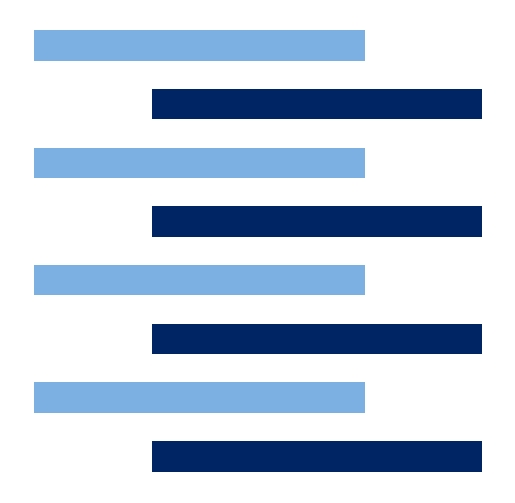
\includegraphics[width=4em]{HAW_wuerfel}}\hspace{1ex}
\parbox[b]{11.2cm}{\sffamily\large%
Hochschule für Angewandte Wissenschaften Hamburg\\[-0.2ex]
Fakultät Design, Medien und Information\\[-0.2ex]
Department Medientechnik
}\\[6ex]
\sffamily\large Erstprüfer: \erstpruef\\[0.5ex]
\sffamily\large Zweitprüfer: \zweitpruef}

%%%%%%%%%%%%%%%%%%%%%%%%%%%%%%%%%%%%%%%%%%%%%%%%%

%---------------------------- Titeldefinitionen --------------------------------------

\newcommand{\vorname}{Sebastian}
\newcommand{\nachname}{Bohn}
\newcommand{\matrikelnummer}{2036605}

\newcommand{\titel}{Analyse und Evaluierung von plattformübergreifenden Spiel-Engines und Frameworks, anhand der Implementierung einer mobilen Beispielapplikation}

\newcommand{\erstpruef}{Prof. Dr. Edmund Weitz}
\newcommand{\zweitpruef}{Prof. Dr. Andreas Plaß}

\date{vorläufige Fassung vom \today}   % Vorab-Version 
%\date{\sffamily Hamburg, DD. MM. YYYY}  % Abgabedatum!

%----------------------------- ANFANG --------------------------------------

\begin{document}
\selectlanguage{ngerman}
\setlength{\parindent}{0em}
% Titelseite erzeugen
\maketitle
% Inhaltsverzeichnis erzeugen          
\tableofcontents
% Seitenumbruch
\clearpage

%----------------------------INHALT---------------------------------------

%---------------------------ABSTRACT------------------------------------
\onehalfspacing
\thispagestyle{empty}
\selectlanguage{english}
\section*{\centering\abstractname}
The market for mobile devices such as smartphones and tablets, regularly improves their technological standards and experience continuous growth for years. 
Due to high usability, mobile devices enjoy great popularity among all kind of consumers. Through the broad quantity of users with high-performance mobile computers, digital games are earning greater popularity than ever. The category Games dominates the amount of downloads of the application stores in all leading systems. In order to meet the demands of users with different systems in an economical way, developers require efficient tools for game development.

\bigskip
These special frameworks and engines for cross-platform game development are reviewed due to their specifications at first step and next through the implementation of an example application applied in practice. By theoretical and practical gained knowledge and the conclusive comparison, it can be evaluated that the choice of the right development tool still largely depends on the requirements. However can Unity3D clearly dominate in most disciplines his competitors and stand out as an all-rounder in game development.


\selectlanguage{ngerman}
\section*{\centering\abstractname}
Der Markt für mobile Geräte, wie Smartphones und Tablets, erfährt seit Jahren kontinuierliches Wachstum und übertrifft regelmäßig seine technologischen Standards. Durch die hohe Benutzerfreundlichkeit erfreuen sich mobile Geräte großer Beliebtheit innerhalb aller Verbraucherschichten. Aufgrund der breiten Masse an Nutzern der performanten Alleskönner, gewinnen auch digitale Spiele immer größere Popularität. Die Kategorie Spiele dominiert die Downloadzahlen der Stores für Applikationen in allen führenden Systemen. Um die Nachfrage für Nutzer unterschiedlicher Systeme auf ökonomische Weise decken zu können, bedarf es entwicklerseitig effizienter Werkzeuge zur Spieleentwicklung.

\bigskip
Diese besonderen Frameworks und Engines für die plattformübergreifende Spieleentwicklung, werden zunächst aufgrund ihrer Spezifikation begutachtet und daraufhin durch die Implementierung einer Beispielapplikation praktisch angewandt. Durch die gewonnenen theoretischen und praktischen Erkenntnisse und den abschließenden Vergleich, kann evaluiert werden, dass die Wahl des passenden Entwicklungstools primär in Abhängigkeit der gestellten Anforderung steht. Jedoch kann Unity3D in den meisten Disziplinen seine Konkurrenz klar dominieren und sich nahezu als Alleskönner der Spieleentwicklung hervorheben.


%----------------------------TEXT-----------------------------------------------

%TODO: Kapitel 1
\chapter{Einleitung}

\section{Motivation}
%TODO: Definition mobile App und Definition eines Spiels
\section{Gliederung}
Die Thesis \emph{„Analyse und Evaluierung von plattformübergreifenden Spiel-Engines und Frameworks, anhand der Implementierung einer mobilen Beispielapplikation“} ist in zehn Kapitel unterteilt, die das Thema systematisch aufbauen und analysieren.

\bigskip
Im ersten Kapitel wird die Motivation für diese Arbeit begründet, sowie die Gliederung für die Vorgehensweise beschrieben.

\bigskip
Das zweite Kapitel analysiert die aktuelle Marktsituation des mobilen Sektors, um die meist genutzten Systeme zu ermitteln. Daraufhin werden durch Statistiken ermittelt, wie das Verhältnis der Downloads an mobilen Spielen gegenüber anderen Kategorien aussieht. Weiterhin werden die Spezifikationen der mobilen Betriebssysteme betrachtet und verglichen. 

\bigskip
Das dritte Kapitel befasst sich mit der nativen Softwareentwicklung von Android, iOS und Windows Phone. Dabei werden die Voraussetzungen, Notwendigkeiten und Möglichkeiten dargelegt.

\bigskip
Die Aspekte der plattformübergreifenden Entwicklung werden im vierten Kapitel behandelt. Dabei werden die generellen Ziele genannt und die verschiedenen Ansätze zur Umsetzung erläutert. 

\bigskip
Im fünften Kapitel werden plattformübergreifende Werkzeuge zur Spieleentwicklung betrachtet. Dafür werden Anforderungen definiert, um Tools zu bestimmen, die vergleichbare Eigenschaften für die Entwicklung mobiler Spiele besitzen. Die ausgewählten Werkzeuge werden daraufhin vorgestellt.

\bigskip
Das sechste Kapitel analysiert die spezifischen Eigenschaften der Spieleframeworks. Dies zeigt die erreichbaren Zielplattformen, die nutzbaren Programmiersprachen, Entwicklungsumgebungen, sowie die Schnittstellen für native Gerätefunktionen und Game Services. Als letztes werden eventuelle Produktvarianten aufgelistet.

\bigskip
Die Konzeption und darauf folgende Implementierung der Beispiel-Applikation ist Thema des siebten Kapitels. Dafür werden zuerst Anforderungen an ein beispielhaftes, mobiles Spiel definiert. Danach wird die gewählte Spielidee und der Spielfluss erklärt. Weiterhin werden die verwendeten Betriebssysteme, Werkzeuge und Versionen aufgelistet. Danach werden die eingesetzten Game Elemente und ihre Verwendung erklärt.

\bigskip
Im achten Kapitel werden die erzeugten Applikationen analysiert. Dafür werden als erstes messbare Metriken definiert, um die Anwendungen zu vergleichbar zu machen. Danach werden die genutzten Testgeräte und die vorgenommenen Grundeinstellungen aufgezeigt. Die Messprotokolle mit den dokumentierten Ergebnissen werden im letzten Teil aufgelistet.

\bigskip
Das neunte Kapitel befasst sich mit dem Vergleich der gewonnenen Erkenntnisse aus den Analysen und der Messresultate. Dafür werden verschiedene Szenarien vorgestellt, die Ausgangssituationen zeigen und zu Entscheidungen für ein zweckmäßiges Entwicklungstool führen.

\bigskip
Das finale Kapitel gibt ein abschließendes Fazit zu der gesamten Arbeit ab.

%Kapitel 2
\chapter{Mobile Systeme}
%TODO Einleitung Kapitel

\section{Marktanalyse zur Gewichtung der mobilen Systeme und der Applikationen}
Welche mobilen Systeme derzeit am meisten gefragt und verbreitet sind, soll in diesem Abschnitt analysiert werden. Dieses Wissen ist nötig, um vor dem Entwicklungsprozess die erfolgreichsten und erfolgversprechendsten Plattformen auszuwählen und miteinzubeziehen.
Weiterhin soll geklärt werden wie viele Applikationen diese Plattformen in ihren Stores bereitstehen und wie die Kategorien gewichtet sind.

\subsection{Marktanteile der mobilen Betriebssysteme}
\label{subsec:Marktanteile_mobile_Systeme}
Eine Statistik über die Marktanteile der mobilen Betriebssysteme bei Smartphones, soll veranschaulichen welche Systeme aktuell zu den führenden gehören. Zusätzlich wird eine zukünftige Verteilung prognostiziert. Die Darstellungen beziehen sich auf Daten der International Data Corporation (IDC), über den globalen Absatz von Smartphones und wurde im August 2015 veröffentlicht. (Abb. \ref{graph_mobile_systems})

\begin{figure}[htbp]
	\centering
	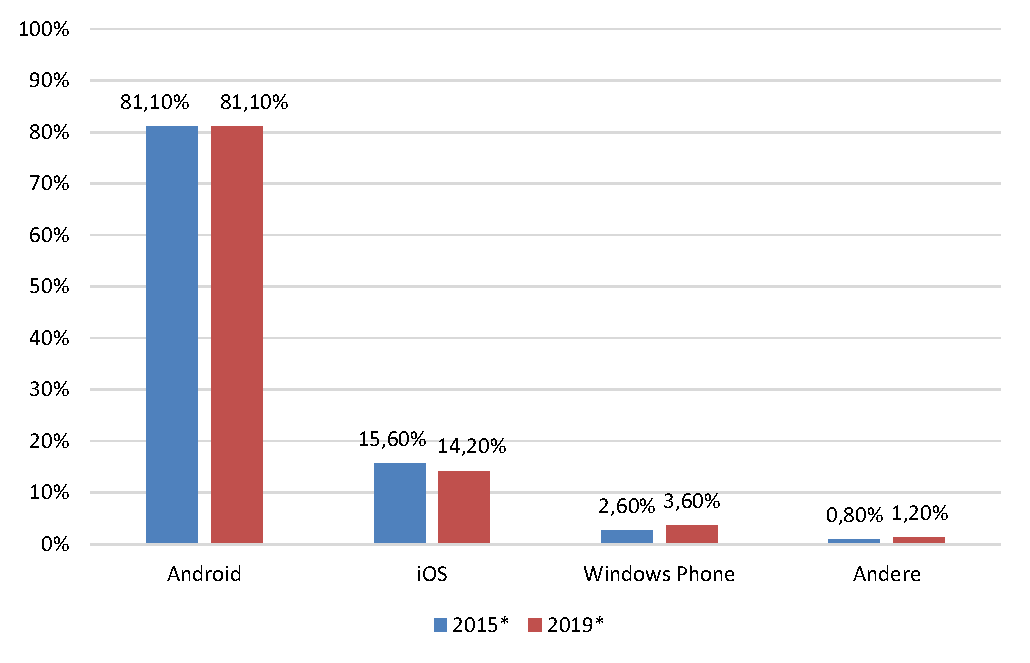
\includegraphics[width=0.8\textwidth]{Bilder/Marktanteile_Betriebssysteme}
	\caption{Prognose zu den Marktanteilen der Betriebssysteme am Absatz vom Smartphones weltweit in den Jahren 2015 und 2019}\label{graph_mobile_systems}\citep{marktanteile_betriebssysteme}
\end{figure}

Die Grafik verdeutlicht, dass aktuell Geräte mit Android Systemen den Markt eindeutig dominieren. Darauf folgen Geräte mit iOS und Windows Phone. Laut Prognose wird sich auch in den nächsten Jahren an dieser Hierarchie nichts ändern. Schlussfolgernd sind diese drei Systeme die relevantesten auf dem globalen Markt.

Abbildung \ref{graph_mobile_systems_laender} gibt Aufschluss über die Verteilung der Systeme nach ausgewählten Ländern. Die Daten beziehen sich auf die Verkäufe von August bis Oktober 2015, welche von Kantar im Dezember 2015 veröffentlicht wurden. Bei der Internationalisierung von Applikationen ist es von Vorteil zu wissen, wie stark die Gewichtung der Systeme in den einzelnen Ländern ist.

\begin{figure}[htbp]
	\centering
	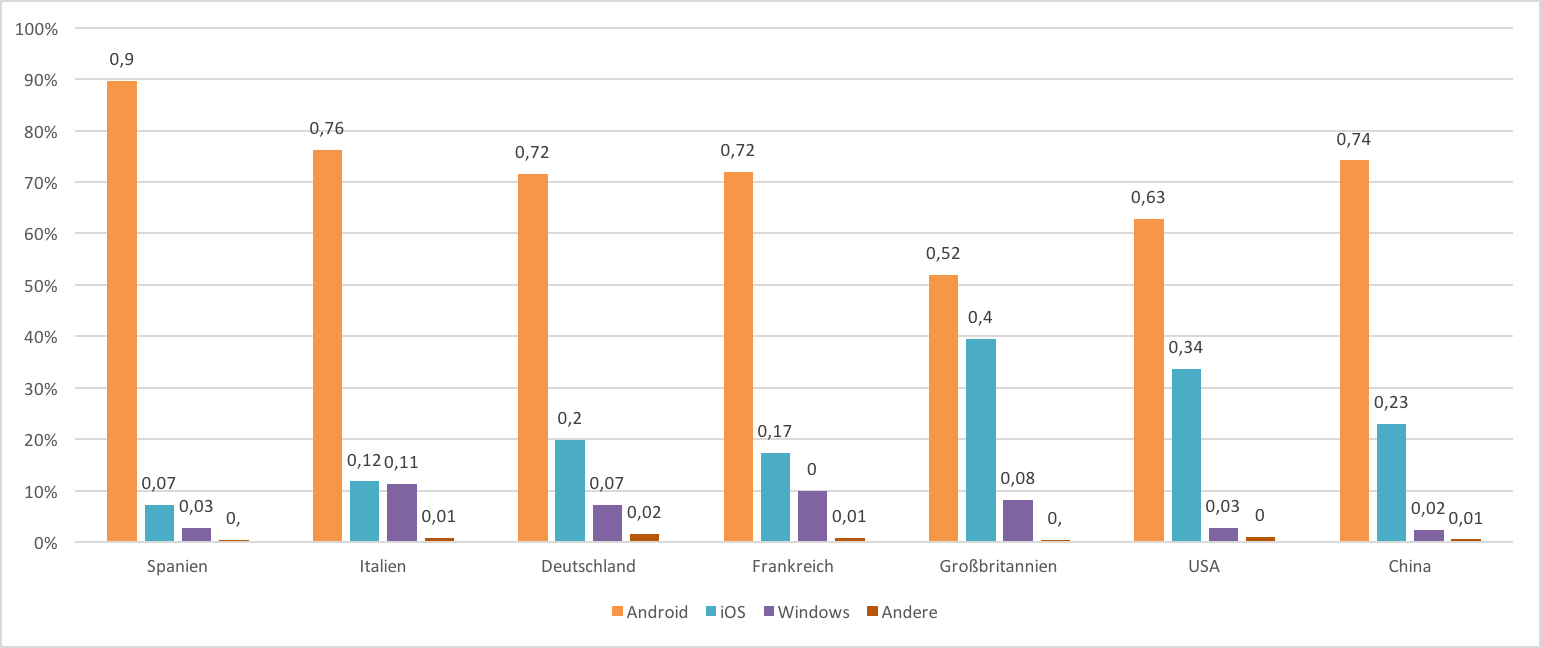
\includegraphics[width=1\textwidth]{Bilder/Marktanteile_nach_Laendern}
	\caption{Marktanteile der mobilen Betriebssysteme am Absatz von Smartphones in ausgewählten Ländern von August bis Oktober 2015}\label{graph_mobile_systems_laender}\citep{marktanteile_betriebssysteme_laender}
\end{figure}

\subsection{Verfügbare Applikationen und Kategorien der Stores}
Die Menge an verfügbaren Apps in den jeweiligen Stores ist unterschiedlich groß.
Eine Analyse über die aktiven Applikationen in den einzelnen Stores und die Gewichtung der Kategorien, soll einen Überblick verschaffen was die jeweiligen Plattformen aktuell zu bieten haben.
In Abbildung \ref{graph_apps_in_stores} wird die Menge an verfügbaren Apps im Mai 2015 dargestellt. Um eine bessere Übersicht zu gewährleisten, wurden die Werte gerundet. Der Amazon Appstore bietet wie der Google Play Store nur Android Apps an. Da es in diesen beiden Stores zum Teil zu Überschneidungen beim Angebot von Anwendungen kommt, werden diese Werte separat betrachtet und nicht summiert.

\begin{figure}[htbp]
	\centering
	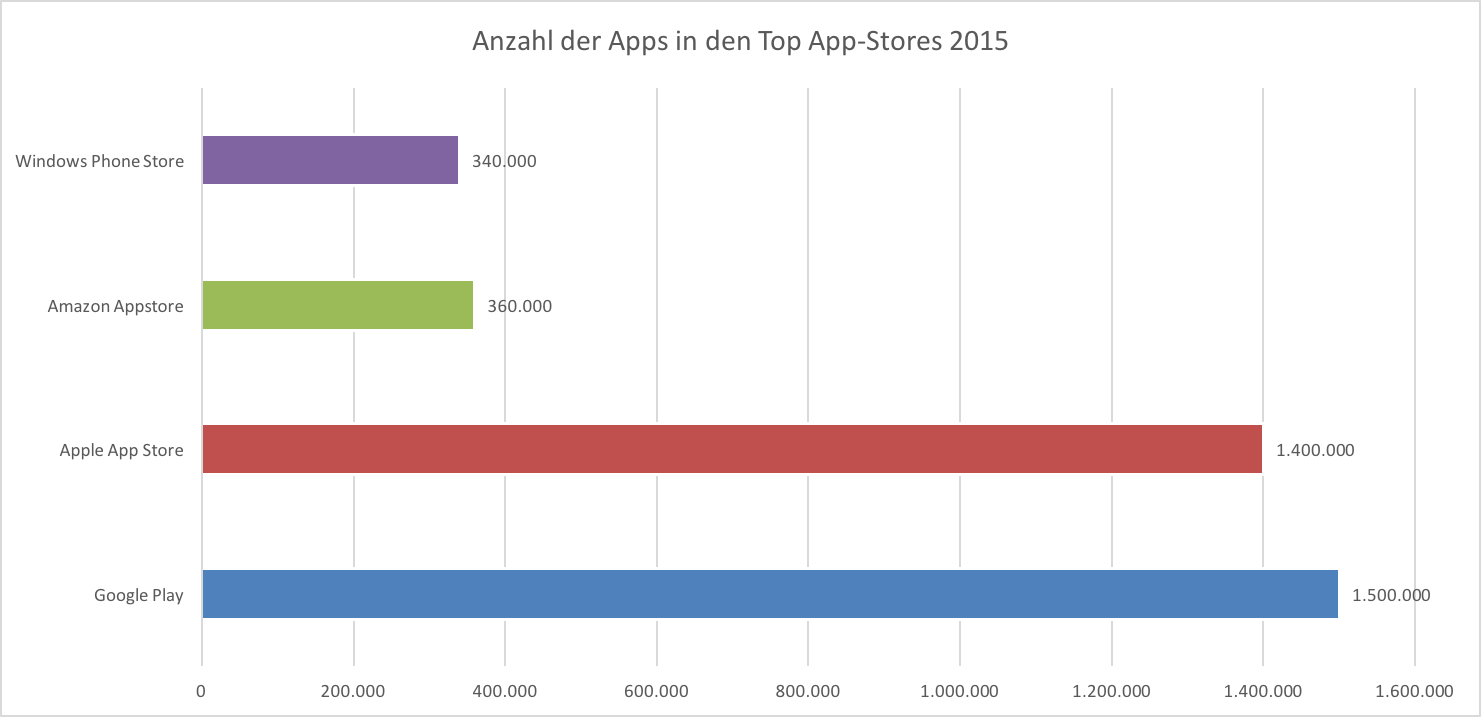
\includegraphics[width=0.8\textwidth]{Bilder/Anzahl_der_Apps}
	\caption{Anzahl der angebotenen Apps in den Top App-Stores im Mai 2015}\label{graph_apps_in_stores}\citep{apps_in_stores}
\end{figure}

Der Wert für den Windows Phone Store ist der Quelle nach von September 2014 und schließt damit noch nicht die Windows 10 Universal Apps mit ein. Diese kamen erst Mitte 2015 dazu und werden in einem getrenntem Windows Store hardwareübergreifend angeboten. Im September 2015 waren rund 80\% der Downloads aus dem Windows Phone Store von Geräten mit der Version 8.1, etwa 15\% von 8.0 Benutzern und etwa 5\% von der aussterbendem Version 7.8.
Laut Windows wurden im September 2015 etwa 50\% der Applikationen mit Windows 10 aus dem neuen Windows Store heruntergeladen. Diese Statistik gibt jedoch wenig Aufschluss wie groß dabei der Anteil an mobilen Systemen ist. Jedoch dominiert die Kategorie "Games" bei Windows 10 Apps mit fast 45\% die Downloadzahlen.\citep{windows_store_trends_2015}

\begin{figure}[htbp]
	\centering
	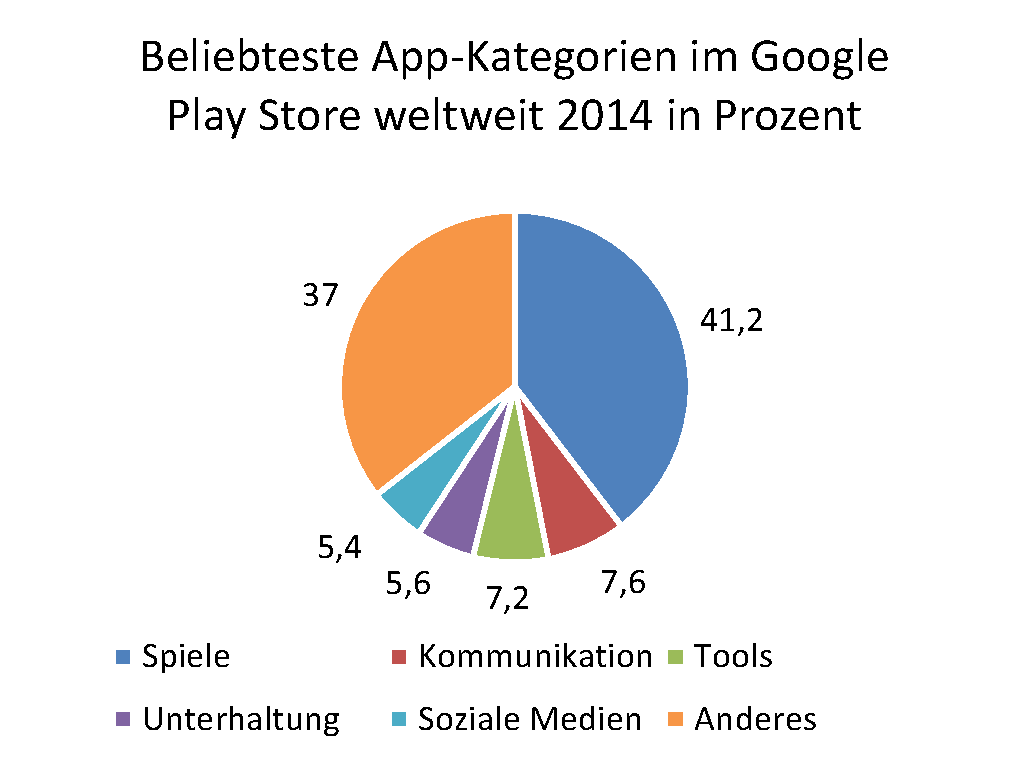
\includegraphics[width=0.6\textwidth]{Bilder/Google_Play_Store_Kategorien}
	\caption{Anteil der im Google Play Store weltweit am häufigsten heruntergeladenen Apps nach Kategorien im Februar 2014}\label{graph_play_store_kategorien}\citep{play_store_categories}
\end{figure}

Auch im Google Play Store werden Spiele Apps am häufigsten heruntergeladen und nehmen etwa 41\% des Downloadvolumens ein.(Abb. \ref{graph_play_store_kategorien})

\begin{figure}[htbp]
	\centering
	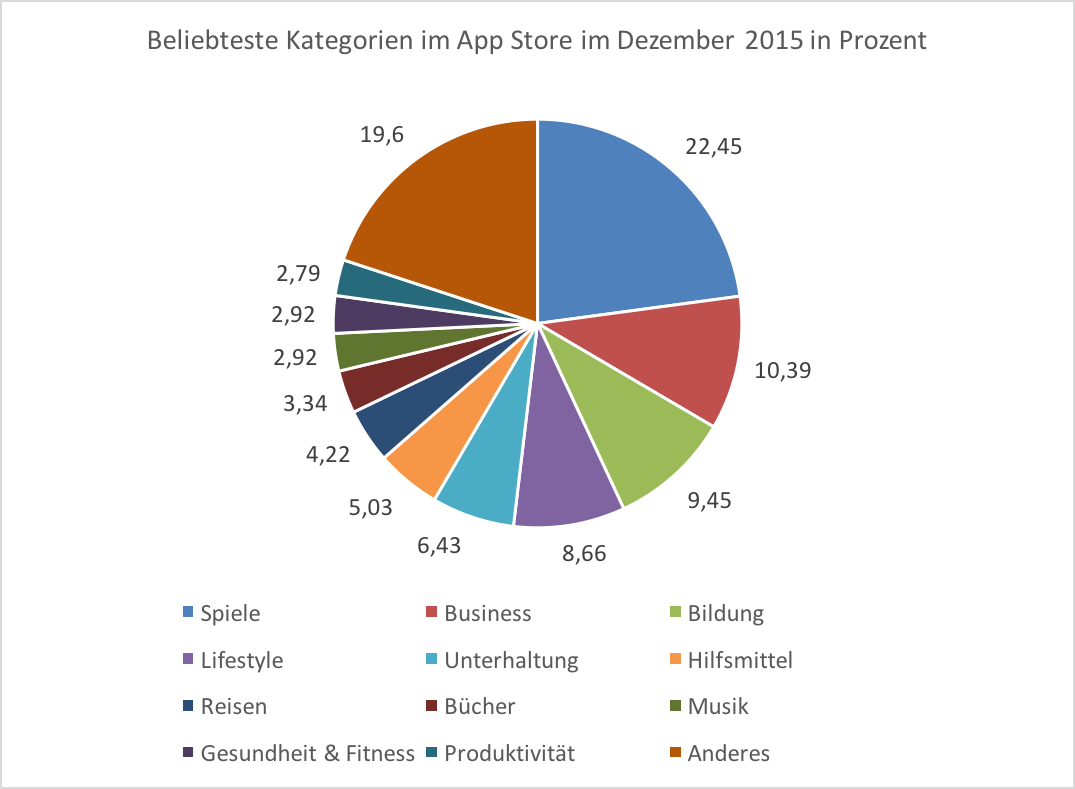
\includegraphics[width=0.8\textwidth]{Bilder/Top_Kategorien_App_Store}
	\caption{Ranking der Top-Kategorien im App Store im Dezember 2015}\label{graph_app_store_kategorien}\citep{app_store_categories}
\end{figure}

Die beliebtesten Kategorien des Apple App Store werden ebenfalls deutlich von den Spielen angeführt. Auch wenn der Abstand zur zweithäufigsten Kategorie geringer ist als bei den anderen Stores, macht der Spielebereich trotzdem etwa ein viertel aller Downloads aus.(Abb. \ref{graph_app_store_kategorien})
\bigskip

Auch wenn jeder Store seine Applikationen auf eigene Weise kategorisiert, ist dennoch klar zu erkennen das Spiele bei jedem Anbieter das höchste Downloadvolumen ausmachen und sich stetig wachsender Beliebtheit erfreuen. Die Nachfrage nach mobilen Spielen ist demnach plattformübergreifend und berechtigt die Evaluierung von entsprechender Entwicklungssoftware.

\section{Betrachtung der mobilen Systeme}
Anhand der gewonnenen Erkenntnisse aus Kapitel \ref{subsec:Marktanteile_mobile_Systeme}, spielen derzeit die mobilen Systeme von Android, iOS und Windows Phone die größte Rolle auf dem Markt und bei den Benutzern. Folglich werden weitere Systeme nicht weiter betrachtet und der Fokus auf diese drei Systeme gerichtet.

\subsection{Android}
Android ist ein Open Source Betriebssystem und gleichzeitig eine Software-Plattform, welches stark im mobilen Bereich vertreten ist und auf dem Linux-Kernel basiert. Zu finden ist diese auf Smartphones, Tablet-Computern, Netbooks und auch auf Smart-TV Geräten. \citep{android_overview} Entwickelt wird Android von der Open Handset Alliance (OHA), welche von Google gegründet wurde. Die OHA wurde im November 2007 gegründet und ist ein Konsortium von mehr als 80 Unternehmen aus den Bereichen Mobilfunknetz, Geräteherstellung, Halbleiterindustrie, Marketing und Software. \citep{alliance_members} Der Grund für die Entwicklung von Android war und ist es, einen offenen Standard für mobile Geräte zu schaffen. \citep{alliance_overview}

Durch sein offenes System ermöglicht Android Entwicklern große Freiheit bei der Programmierung von Applikationen. Eigene Entwicklungen können auch mit Anwendungen von Google, wie zum Beispiel Google Maps, verknüpft werden.

Auch der Hardwarebereich bietet ein breites Spektrum an Geräten mit kostengünstigen, bis hochpreisigen Angeboten, sowohl mit einfacher bis qualitativ hochwertiger, technischer Ausstattung. Benutzer haben die Möglichkeit, ihre Geräte weitestgehend frei zu gestalten und einzustellen. Für die Installation von neuen Applikationen sind diese auch nicht an einen einzigen Store gebunden und können Apps auch aus verschiedensten Quellen beziehen.
\\

Vorteile:
\begin{itemize}
	\item Open Source
	\item Unabhängigkeit von Anbietern
	\item Personalisierung
	\item Hardwareangebot
\end{itemize}

Nachteile:
\begin{itemize}
	\item Hohe Verbreitung von Schadsoftware
	\item Aktualität der Version ist abhängig vom Gerätehersteller
\end{itemize}

\subsection{iOS}
iOS ist das mobile Betriebssystem des Unternehmen Apple. Dieses ist ein Derivat von Mac OS X, welches selbst auf Unix basiert. Es wird ausschließlich von Apple entwickelt und ist somit nur auf den eigenen Geräten iPhone, iPad und iPod touch zu finden. Mit der Entwicklung wurde unter externer und interner Geheimhaltung 2005 begonnen und das Resultat der Öffentlichkeit zum ersten Mal Anfang 2007 vorgestellt. Bis zur Version 4.0 wurde iOS mit dem Namen iPhoneOS betitelt. Das Konzept und Design ist schwerpunktmäßig auf hohe Benutzerfreundlichkeit und Funktionalität ausgelegt. 

Durch die geschlossene Struktur des Systems sind eigene Derivate nicht möglich. Benutzer sind für den offiziellen Bezug von Applikationen auf Apples App Store angewiesen.
Bei der Wahl der Hardware ist man auf die Produktpalette von Apple angewiesen, welche jährlich eine neue Generation veröffentlicht. Die Personalisierung der Geräte ist nur bedingt möglich, da Anbieter von Drittsoftware keinen Zugriff auf das System haben und Anwendungen nur offiziell über den eigenen App Store bezogen werde können. Dies bietet jedoch den Vorteil einer Qualitätssicherung durch Apple, da Applikationen vor der Veröffentlichung einer Prüfung unterzogen werden.
\\

\textbf{Vorteile:}
\begin{itemize}
	\item Kompatibilität von Software und Hardware
	\item Benutzerfreundlichkeit
	\item Geräteübergreifende Kommunikation
	\item Kontrollen bei Veröffentlichung von Anwendungen
\end{itemize}

\textbf{Nachteile:}
\begin{itemize}
	\item Restriktive Firmenpolitik
	\item Proprietäres System
	\item Hardwareauswahl
	\item Anwendungen nur über den App Store
\end{itemize}

\subsection{Windows Phone}
Entwickler Microsoft stellt seit dem Jahr 2000 Betriebssysteme für mobile Geräte her. \citep{microsoft_mobile} 
Seitdem hat sich die Namensgebung von Windows Mobile, über Windows Phone, bis zum aktuellsten Windows 10 Mobile vorgearbeitet. Um im allgemeinen Bezug nicht zwischen den Namen hin und her zu wechseln, wird in dieser Arbeit, wenn mobile Windows Systeme erwähnt werden, der Name Windows Phone (oder WP) benutzt.
Die frühen Versionen von Windows Phone, also Windows Mobile und Windows Phone 7 stammen noch von dem Windows CE Kernel ab, wobei die aktuellen Versionen, Windows Phone 8 und Windows 10 Mobile, Derivate des Windows NT Kernels sind. Mit dem neuesten Ableger, Windows 10 Mobile, verspricht Microsoft eine homogene Kommunikations- und Anwendungsstruktur zwischen allen Geräten die mit diesem System betrieben werden. Dazu zählen nicht nur Smartphones und Tablets, sondern auch Notebooks, Desktop PCs und die Spielkonsole Xbox One. \citep{windows10_features}

Microsoft verfolgt mit Windows Phone eine ähnlich geschlossene und proprietäre Struktur wie der Konkurrent Apple. Eigene Derivate des Systems sind also nicht offiziell möglich. Auch die Benutzer müssen für neue Anwendungen auf das Angebot des Windows Stores zurückgreifen. Jedoch will Microsoft Entwicklern die Möglichkeit bieten, zukünftige Anwendungen universell verfügbar zu machen, das diese auf allen Windows Systemen nutzbar sind. Microsoft arbeitet außerdem an einer Technik, die bestehende Android und iOS Anwendungen auf die Windows Plattform überführen kann. \citep{wp_with_android_ios}

Die aktuellen Windows Phone Versionen sind durch eine Allianz von Windows und Nokia, hauptsächlich auf mobilen Geräten von Nokia zu finden.\citep{microsoft_nokia}
Aber auch andere Hersteller bieten Geräte mit Windows Phone, jedoch bisher in einem überschaubaren Umfang.
\\

Vorteile:
\begin{itemize}
	\item Kompatibilität von Software und Hardware
	\item Universelle Anwendungen
	\item Benutzerfreundlichkeit
\end{itemize}

Nachteile:
\begin{itemize}
	\item Proprietäres System
	\item Anwendungen nur aus dem Windows Store
	\item Geringeres Angebot an Anwendungen
\end{itemize}
\citep{wp_pros_cons}

%OPTIONAL!!!
%subsection{Weitere Systeme}

\chapter{Native Softwareentwicklung}
Softwareentwicklung für ein bestimmtes System wird als nativ (lat.: angeboren, natürlich) bezeichnet. Hier sind Dateiformate, Programmiersprachen, Hardware, Entwicklungsumgebungen und Kompilierung genau an die Zielplattform angepasst. Nativer Code ist in der Lage alle individuellen Eigenschaften einer Zielplattform anzusprechen, ohne dabei eine eventuelle Portierbarkeit zu berücksichtigen.
\citep{native_software}
Welche Anforderungen iOS, Android und Windows Phone bezüglich nativer Entwicklung voraussetzen, soll in diesem Kapitel näher erläutert werden.

\section{Systemvoraussetzungen}
Um Applikationen für eine bestimmte Zielplattform zu entwickeln, werden unter Umständen Voraussetzungen an das Betriebssystem des Entwicklers gestellt.

\subsection{Android}
Die Entwicklung von Android Applikationen ist an kein bestimmtes System gebunden. Somit lassen sich diese unter Windows, OS X und Linux Systemen entwickeln. Dies wird unter anderem durch die Eigenschaften der Programmiersprache Java ermöglicht.
Windows Benutzer sollten mindestens Windows XP nutzen. Darüber hinaus können alle aktuelleren Versionen genutzt, wobei alle 32-Bit Editionen unterstützt werden. Ab Windows 7 wird 64-Bit ebenfalls unterstützt.
Mac Systeme werden ab OS X 10.5.8 von den offiziellen Entwicklungswerkzeugen unterstützt.
Um auf einem Linux System zu entwickeln, kann man dies beispielsweise unter Ubuntu ab Version 8.04 tun. Bei 64-Bit Versionen ist es notwendig, dass diese fähig ist 32-Bit Anwendungen auszuführen. Da die Auswahl an Linux-Distributionen sehr umfangreich ist, wird an dieser Stelle auf diese nicht weiter eingegangen.
\citep{android_sdk_requirements}

\subsection{iOS}
Für den reinen Schreibvorgang von iOS Anwendungen ist prinzipiell jedes System geeignet. Jedoch ist es offiziell nur auf einem Apple OS X System möglich, die geschriebene Software zu kompilieren und auf der Zielhardware zu testen. Für Entwickler die kein OS X System ihr Eigen nennen oder keinen Zugang zu solcher haben, besteht die Möglichkeit einen Cloudservice zu nutzen. \textit{MacinCloud} bietet eine cloudbasierte Vermietung von OS X Systemen, inklusive der benötigten Entwicklungssoftware. \citep{macincloud}

\subsection{Windows Phone}
Ähnlich wie bei iOS, wird für die Kompilierung von Windows Phone Applikationen ein passendes Windows System vorausgesetzt. Jedoch sind manche Voraussetzungen leider etwas undurchsichtig. Das bedeutet, dass für die Entwicklung einer Windows Phone 8 App mindestens ein Windows 8 Betriebssystem benötigt wird. Außerdem wird das SDK 8.0 nur von der 64-bit Version unterstützt. Weiter wird beispielsweise für die Nutzung des Simulators eine Windows 8 Pro Version und die Virtualisierungstechnologie Hyper-V benötigt. Das Windows 10 SDK erwartet minimal Windows 7. Der Simulator benötigt die gleichen Mindestanforderungen wie bei Windows 8. \citep{WP8_requirements, WP10_SDK, WP10_Emulator} 

\section{SDKs und Versionen}
Software Development Kits, kurz SDKs, liefern dem Entwickler die Werkzeuge, Anwendungen und bestenfalls eine aktuelle Dokumentation, um für eine bestimmte Zielplattform zu entwickeln. Auch sind sie notwendig, um geschriebenen Code zu interpretieren und kompilieren. Um die aktuellste Version eines mobilen Systems zu unterstützen, muss das SDK auf ebenso aktuellen Stand sein.
\clearpage 

\subsection{Android Versionen}
Android Versionen sind nach süßen Leckereien benannt und dem Anfangsbuchstaben nach alphabetisch aufsteigend. (Abb. \ref{tab_android_vers})
Das aktuelle SDK ist frei im Netz verfügbar. Dieses kann einzeln geladen werden oder direkt in Verbindung mit Android Studio.

\begin{table}[htbp]
	\centering
	\resizebox{1\textwidth}{!}{%
		\begin{tabular}{|c|c|c|c|}
			\hline
			\rowcolor[HTML]{000000} 
			{\color[HTML]{FFFFFF} \textbf{Codename}} & {\color[HTML]{FFFFFF} \textbf{Version}} & {\color[HTML]{FFFFFF} \textbf{API Level}} & {\color[HTML]{FFFFFF} \textbf{Erscheinungsdatum}} \\ \hline
			Marshmallow                              & 6                                       & 23                                        & 5. Oktober 2015                                   \\ \hline
			Lollipop                                 & 5.1.x                                   & 22                                        & 9. März 2015                                      \\ \hline
			Lollipop                                 & 5.0.x                                   & 21                                        & 3. November 2014 - 19. Dezember 2014              \\ \hline
			Wear                                     & 4.4W                                    & 20                                        & Juni 2014                                         \\ \hline
			KitKat                                   & 4.4.x                                   & 19                                        & 31. Oktober 2013 - 19. Juni 2014                  \\ \hline
			Jelly Bean                               & 4.3.x                                   & 18                                        & 24. Juli 2013 - 4. Oktober 2013                   \\ \hline
			Jelly Bean                               & 4.2.x                                   & 17                                        & 13. November 2012 - 12. Februar 2013              \\ \hline
			Jelly Bean                               & 4.1.x                                   & 16                                        & 27. Juni 2012 - 10. Oktober 2012                  \\ \hline
			Ice Cream Sandwich                       & 4.0.3 - 4.0.4                           & 15, NDK 8                                 & 16. Dezember 2011 - 4. Februar 2012               \\ \hline
			Ice Cream Sandwich                       & 4.0 - 4.0.2                             & 14, NDK 7                                 & 19. Oktober 2011 - 15. Dezember 2011              \\ \hline
			Honeycomb                                & 3.2.x                                   & 13                                        & 16. Juli 2011                                     \\ \hline
			Honeycomb                                & 3.1                                     & 12, NDK 6                                 & 10. Mai 2011                                      \\ \hline
			Honeycomb                                & 3                                       & 11                                        & 23. Februar 2011                                  \\ \hline
			Gingerbread                              & 2.3.3 - 2.3.7                           & 10                                        & 23. Februar 2011 - 20. September 2011             \\ \hline
			Gingerbread                              & 2.3 - 2.3.2                             & 9, NDK 5                                  & 6. Dezember 2010 - Januar 2011                    \\ \hline
			Froyo                                    & 2.2 - 2.2.2                             & 8, NDK 4                                  & 20. Mai 2010 - Januar 2011                        \\ \hline
			Eclair                                   & 2,1                                     & 7, NDK 3                                  & 12. Dezember 2010                                 \\ \hline
			Eclair                                   & 2.0.1                                   & 6                                         & 3. Dezember 2009                                  \\ \hline
			Eclair                                   & 2                                       & 5                                         & 26. Oktober 2009                                  \\ \hline
			Donut                                    & 1.6                                     & 4, NDK 2                                  & 15. September 2009                                \\ \hline
			Cupcake                                  & 1.5                                     & 3, NDK 1                                  & 30. April 2009                                    \\ \hline
			ohne Codename                            & 1.1                                     & 2                                         & 10. Februar 2009                                  \\ \hline
			ohne Codename                            & 1                                       & 1                                         & 23. September 2008                                \\ \hline
		\end{tabular}
	}
	\caption{Android Versionen und ihr Erscheinungsdatum}\label{tab_android_vers}\citep{android_codenames,android_version_releases}
\end{table}
\clearpage

\subsection{iOS Versionen}
Apple nutzt für seine Produkte Codenamen, die keinem bestimmten Muster folgen. Verbrauchern sind diese meist unbekannt, da diese überwiegend intern genutzt werden. (Abb. \ref{tab_ios_vers})
Das SDK wird offiziell ausschließlich in Verbindung mit XCode bezogen.
 
\begin{table}[htbp]
	\centering
	\resizebox{0.6\textwidth}{!}{%
		\begin{tabular}{|c|c|c|}
			\hline
			\rowcolor[HTML]{000000} 
			{\color[HTML]{FFFFFF} \textbf{Codename}} & {\color[HTML]{FFFFFF} \textbf{Version}} & {\color[HTML]{FFFFFF} \textbf{Erscheinungsdatum}} \\ \hline
			Monarch                                  & 9.2 Beta                                & 3. November 2015                                  \\ \hline
			Monarch                                  & 9.1                                     & 21. Oktober 2015                                  \\ \hline
			Monarch                                  & 9.0.x                                   & 16. September 2015                                \\ \hline
			Copper                                   & 8.4.x                                   & 30. Juni 2015                                     \\ \hline
			Stowe                                    & 8.3                                     & 8. April 2015                                     \\ \hline
			OkemoZurs                                & 8.2                                     & 9. März 2015                                      \\ \hline
			OkemoTaos                                & 8.1.x                                   & 9. Dezember 2015                                  \\ \hline
			Okemo                                    & 8.0.x                                   & 17. September 2014                                \\ \hline
			Sochi                                    & 7.1.x                                   & 10. März 2014                                     \\ \hline
			Innsbruck                                & 7.0.x                                   & 18. September 2013                                \\ \hline
			Brighton                                 & 6.1.x                                   & 21. Februar 2013                                  \\ \hline
			Sundance                                 & 6.0.x                                   & 19. September 2012                                \\ \hline
			Hoodoo                                   & 5.1.x                                   & 7. März 2012                                      \\ \hline
			Telluride                                & 5.0.x                                   & 12. Oktober 2011                                  \\ \hline
			Durango                                  & 4.3.x                                   & 9. März 2011                                      \\ \hline
			Jasper                                   & 4.2.x                                   & 22. November 2010                                 \\ \hline
			Baker                                    & 4.1                                     & 8. September 2010                                 \\ \hline
			Apex                                     & 4.0.x                                   & 21. Juni 2010                                     \\ \hline
			Wildcat                                  & 3.2.x                                   & 3. April 2010                                     \\ \hline
			Northstar                                & 3.1.x                                   & 9. September 2009                                 \\ \hline
			Kirkwood                                 & 3.0.x                                   & 17. Juni 2009                                     \\ \hline
			Timberline                               & 2.2.x                                   & 21. November 2008                                 \\ \hline
			Sugarbowl                                & 2.1.x                                   & 9. September 2008                                 \\ \hline
			Big Bear                                 & 2.x                                     & 11. Juli 2008                                     \\ \hline
			Little Bear                              & 1.1.x                                   & 14. September 2007                                \\ \hline
			Alpine                                   & 1.0.x                                   & 29. Juni 2007                                     \\ \hline
		\end{tabular}
	}
\caption{iOS Versionen und ihr Erscheinungsdatum}\label{tab_ios_vers}\citep{ios_codenames}
\end{table}

\subsection{Windows Phone Versionen}
Tabelle \ref{tab_WP_versions} berücksichtigt alle Versionen ab Windows Phone 7. Die Unterstützung seitens Microsoft wurde bereits eingestellt. Version 8 soll laut Angabe bis etwa 2017 weitergeführt werden, bis die Portierungen der Nutzer zu Windows 10 abgeschlossen sind.

\begin{table}[htbp]
	\centering
	\resizebox{0.7\textwidth}{!}{%
		\begin{tabular}{|c|c|c|}
			\hline
			\rowcolor[HTML]{000000} 
			{\color[HTML]{FFFFFF} \textbf{Codename}} & {\color[HTML]{FFFFFF} \textbf{Version}} & {\color[HTML]{FFFFFF} \textbf{Erscheinungsdatum}} \\ \hline
			Windows Phone 7                          & 7.0.7004.0                              & 21. Oktober 2010                                  \\ \hline
			PreNoDo                                  & 7.0.7008.0                              & 21. Februar 2011                                  \\ \hline
			NoDo                                     & 7.0.7390.0                              & 22. März 2011                                     \\ \hline
			& 7.0.7392.0                              & 3. Mai 2011                                       \\ \hline
			& 7.0.7403.0                              & September 2011                                    \\ \hline
			7.5 / Mango                              & 7.10.7720.68                            & 27. September 2011                                \\ \hline
			& 7.10.7740.16                            & 17. November 2011                                 \\ \hline
			& 7.10.8107.79                            & 4. Januar 2012                                    \\ \hline
			& 7.10.8112.7                             & Juni 2012                                         \\ \hline
			7.5 Refresh / Tango                      & 7.10.8773.98                            & 27. Juni 2012                                     \\ \hline
			& 7.10.8779.8                             & 15. August 2012                                   \\ \hline
			& 7.10.8783.12                            & 30. Januar 2013                                   \\ \hline
			7.8                                      & 7.10.8858.136                           & 30. Januar 2013                                   \\ \hline
			& 7.10.8860.142                           & 14. März 2013                                     \\ \hline
			& 7.10.8862.144                           & 15. März 2013                                     \\ \hline
			8.0 / Apollo                             & 8.0.9903.10                             & 29.Oktober 2012                                   \\ \hline
			Portico                                  & 8.0.10211.204                           & 29. Januar 2013                                   \\ \hline
			Apollo+                                  & 8.0.10327.77                            & 19. Juli 2013                                     \\ \hline
			& 8.0.10512.142                           & 14. Oktober 2013                                  \\ \hline
			Blue                                     & 8.10.12397.895                          & 16. Juli 2014                                     \\ \hline
			& 8.10.14234.375                          & 5. Dezember 2014                                  \\ \hline
			& 8.10.15148.160                          & 11. April 2015                                    \\ \hline
			Windows 10                               & 10.0.10586.0                            & 20. November 2015                                 \\ \hline
			& 10.0.10586.29                           & 8. Dezember 2015                                  \\ \hline
		\end{tabular}
	}
	\caption{Windows Phone Versionen und ihr Erscheinungsdatum}
	\label{tab_WP_versions}\citep{WP7_version_releases, WP8_version_releases, WP10_version_releases}
\end{table}

\section{Programmiersprachen}
In der nativen Entwicklung werden für jede Zielplattform bestimmte Programmiersprachen unterstützt. 

\subsection{Android}
Android Applikationen werden in Java entwickelt. Demnach ist es notwendig, zusätzlich eine aktuelle Java Version (JDK) zu installieren. Diese wird von dem Unternehmen Oracle, mit der aktuellen Version 8  vertrieben. In Kapitel \ref{subsec:libGDX} wird nochmal näher auf diese Programmiersprache eingegangen. 
\citep{java_jdk}

\subsection{iOS}
Die primäre Programmiersprache für iOS und OS X ist derzeit die objektorientierte Erweiterung von C, Objective-C. Diese befindet sich aktuell in der Version 2.0. Objective-C wurde weiterhin von der Sprache Smalltalk beeinflusst und leitet zum Beispiel die Syntax dessen Objekteigenschaften ab. Trotzdem besteht weiterhin die Nähe zur C Syntax, in Bezug auf nicht-objektorientierter Operationen. \citep{objectiveC_about}


Alternativ kann die relativ junge Sprache Swift eingesetzt werden. Diese ist ebenfalls objektorientiert und in der aktuellen Version 2.0. Im Dezember 2015 wurde der Quellcode als Open Source zur Verfügung gestellt. Swift soll Objective-C allerdings nicht ersetzen, sondern eine weitere Möglichkeit darstellen. Die beiden Sprachen sind miteinander kompatibel, so dass es möglich beide in demselben Projekt zu nutzen.
\citep{swift_about}

\subsection{Windows Phone}
Für die Benutzeroberfläche wird hauptsächlich die Sprache XAML (Extensible Application Markup Language) genutzt. Um die Logik zu erstellen, hat der Entwickler die Freiheit C\#, Visual Basic, JavaScript oder C++ nutzen.

\section{Entwicklungsumgebungen}
Für die Entwicklung werden jeweilig verschiedene IDEs (Integrated Development Environment) seitens der Betreiber unterstützt und empfohlen. Eine Besonderheit bei IDEs für mobile Systeme ist die Unterstützung eines Simulators. Dieser simuliert ein spezifiziertes Gerät auf virtuelle Weise, um Entwicklungen direkt testen zu können.

\subsection{Android}
Android empfiehlt das eigene Android Studio, welches die offizielle IDE für Android Entwicklung darstellt und zusätzlich das aktuelle SDK mitliefert. Android Studio basiert auf der IDE IntelliJ IDEA und ist frei verfügbar.\citep{android_studio} Alternativer Vorgänger ist die quelloffene IDE Eclipse.

\subsection{iOS}
Xcode ist die IDE von Apple, ohne die keinerlei Kompilierung von iOS Projekten möglich ist.
Diese befindet sich derzeit in der stabilen Version 7 und liefert das benötigte SDK, so wie einen umfangreichen Simulator mit allen mobilen Apple Geräten. Xcode ist verpflichtend, wenn die geschriebene Anwendung auf einer realen Hardware getestet werden soll. Seit dem 3. Quartal 2015 ist dafür auch keine kostenpflichtige Entwicklerlizenz nötig, sondern fällt nur noch bei einem Release im App Store an. 
\citep{t3n_xcode7}
Eine alternative bietet JetBrains IDE Appcode, welches eine kompatible, aber kostenpflichtige Erweiterung zu Xcode ist.
\citep{appcode}


\subsection{Windows Phone}
Microsoft setzt für die Kompilierung und Realisierung für WP Projekte eine Visual Studio IDE voraus, welche für Entwicklungen außerhalb eines Unternehmens kostenfrei ist.


\section{Native Spieleentwicklung}
Bei der nativen Entwicklung, basieren die mobilen Applikationen auf den jeweiligen SDKs. Mobile Spiele können auf nativem Wege realisiert werden. Die Verwendung der mitgelieferten Grafik- und Animationsfunktionen für die Visualisierung und selbstdefinierte Logik durch eigenen Code, können schon ausreichen, um einfache 2D Spiele zu kreieren. Auch mit der freien Grafikbibliothek OpenGL, könnten Spielinhalte in 2D oder sogar 3D dargestellt werden. Allerdings ist OpenGL nicht für Windows Phone verfügbar, denn hier wird das hauseigene Pendant, DirectX verwendet. Um die Spieleentwicklung leichter zu machen, können spezialisierte Frameworks und Editoren genutzt werden, die eigens für die Entwicklung von Spielen konzipiert wurden und auf die gewünschte Plattform abgestimmt sind. In den folgenden Unterkapiteln werden beispielhafte Werkzeuge für die jeweiligen Plattformen aufgelistet. Bei der Recherche nach spezialisierten Frameworks, war ein gewisser Trend zu verzeichnen. Die Gesamtmenge an Projekten ist groß, wovon aber der Großteil nicht mehr weiterentwickelt wird und die Zahl derer die sich behaupten konnten ist verhältnismäßig gering.
 
\subsection{Android}
Für Android existieren einige Frameworks, wovon jedoch viele nicht immer auf dem neuesten Stand sind. Das ist häufig damit verbunden, dass diese aus privatem Interesse entstanden sind und ein unkommerzielles, kostenloses Vertriebsmodell betreiben. Daher sind regelmäßige Aktualisierungen oft nicht gewährleistet und manche Arbeiten wurden auch ganz eingestellt.

\bigskip
\textbf{AndEngine}\\
Eine Game Engine die auf OpenGL basiert und für 2D Spiele ausgelegt ist.
Die Letzte Aktualisierung erfolgte im Dezember 2013.

\bigskip
\textbf{Cocos2D-Android}\\
Eine Implementierung von Cocos2D für Android. Die Weiterentwicklung wurde allerdings eingestellt und die letzte Änderung erfolgte im Januar 2010.

\bigskip
\textbf{jPCT-AE}\\
Eine 3D Engine die auf jPCT für Desktopanwendungen mit Java basiert und für Android portiert wurde. Die Grafik wird von OpenGL 1.x und 2.0 unterstützt. Das Projekt wird aktuell auch weiterentwickelt und ist frei verfügbar.

\subsection{iOS}
Auch für iOS bestehen diverse Frameworks. Die Suche nach einer aktuellen Entwicklungsunterstützung gestaltet sich hier ein wenig einfacher, wobei man aber genau wie bei Android auch auf aufgegebene Projekte stößt. Ein großer Vorteil besteht aber durch SpriteKit, da dies ein Produkt von Apple selbst ist und eine gewisse Sicherheit bei zukünftiger Unterstützung gewährleistet.

\bigskip
\textbf{SpriteKit}\\
Eigenentwicklung von Apple für 2D Spiele auf iOS und OS X. Es kann Objective-C oder Swift genutzt werden.

\bigskip
\textbf{Cocos2D-iPhone}\\
Abkömmling von Cocos2D für iOS mit den Implementierungen für Objective-C und zukünftig auch Swift. Dies ist einer der Hauptzweige von Cocos2D der stetig aktualisiert wird.

\bigskip
\textbf{Sparrow}\\
Eine aktuelle Open Source Game Engine für iOS Spiele, die ausschließlich Objective-C unterstützt.

\subsection{Windows Phone}
Frameworks die einzig und allein für Windows Phone Spiele ausgelegt sind, waren nicht direkt ausfindig zu machen. Microsoft selbst rät zu dem eigenen XNA Framework, womit auch die meisten Entertainment Plattformen von Microsoft bedient werden können. Hauptsächlich werden hier Cross Plattform Tools genutzt, da die Verbreitung von entsprechender Hardware noch relativ gering ausfällt. Auch durch das neue Windows 10 und der Wunsch zu universellen Anwendungslösungen, besteht derzeit ein noch nicht abgeschlossener Änderungsprozess. Dadurch werden spezialisierte Lösungen für eine Windows Gerätekategorie zukünftig vermutlich eher uninteressant.


\section{Zusammengefasste Übersicht}
Die Tabelle \ref{platform_differnces} soll eine kompaktere Übersicht der einzelnen Systeme bieten.



\begin{table}[htbp]
	\centering
	\resizebox{\textwidth}{!}{%
		\begin{tabular}{cccc}
			\rowcolor[HTML]{000000} 
			{\color[HTML]{FFFFFF} \textbf{Eigenschaft}}         & {\color[HTML]{FFFFFF} \textbf{Android}} & {\color[HTML]{FFFFFF} \textbf{iOS}} & {\color[HTML]{FFFFFF} \textbf{Windows Phone}}     \\
			\cellcolor[HTML]{FFFFFF}\textbf{Virtuelle Maschine} & Dalvik VM                      & -                          & CLR                                      \\
			\rowcolor[HTML]{C0C0C0} 
			\textbf{Programmiersprache}                         & Java                           & Objective-C, Swift         & C\#, C++, Visual Basic, JavaScript, .NET \\
			\cellcolor[HTML]{FFFFFF}\textbf{User Interface}     & XML                            & Cocoa Touch                & XAML                                     \\
			\rowcolor[HTML]{C0C0C0} 
			\textbf{Speicher Management}                          & Garbage collector              & Reference counting         & Garbage collector                        \\
			\cellcolor[HTML]{FFFFFF}\textbf{IDE}                & Eclipse, Android Studio        & Xcode                      & Visual Studio                            \\
			\rowcolor[HTML]{C0C0C0} 
			\textbf{Entwicklungsplattform}                      & Multi-Plattform                & Mac OS X                   & Windows                                  \\
			\cellcolor[HTML]{FFFFFF}\textbf{Geräte}             & Heterogen                      & Homogen                    & Homogen                                  \\
			\rowcolor[HTML]{C0C0C0} 
			\textbf{App Markt}                                  & Google Play Store              & Apple App Store            & Windows Phone Store                     
		\end{tabular}
	}
	\caption{Unterschiede zwischen Android, iOS und Windows Phone}
	\label{platform_differnces}
\end{table}

%OPTIONAL!!!
%\chapter{Stores für mobile Spiele}
%\section{Allgemeine Bedingungen für Entwickler}
%\section{Maximale App-Größe}
%\section{Anforderungen an den Quellcode}
%\section{Kosten und Abgaben}

\chapter{Plattformübergreifende Entwicklung}
Die Entwicklung von Software-Produkten und Services, welche auf mehreren Systemen oder Laufzeitumgebungen funktioniert, wird als plattformübergreifende oder auch Cross-Plattform Entwicklung definiert. Um dies zu gewährleisten nutzen Entwickler unterschiedliche Methoden und Techniken, um verschiedene Systeme mit einer Projektstruktur zu erreichen.\citep{cross_plattform_explanation}

\begin{figure}[htbp]
	\centering
	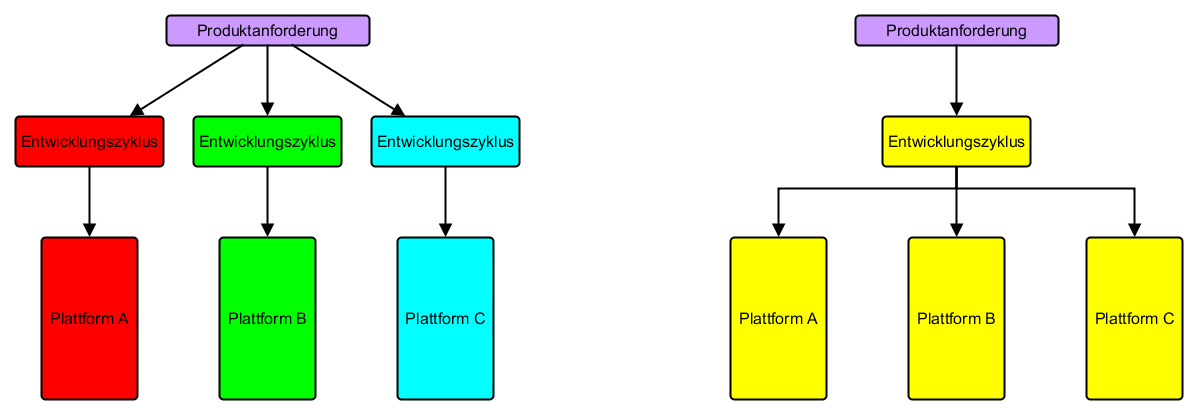
\includegraphics[width=1\textwidth]{Bilder/nativ_vs_cross}
	\caption{Traditionelle und plattformübergreifende Entwicklungsmodelle}\label{graph_nativ_vs_cross}
\end{figure}


\section{Ziel}
Die Idee und das Ziel von plattformübergreifender Entwicklung sind, dass eine Softwareanwendung auf mehr als einer spezifischen digitalen Umgebung zufriedenstellend funktioniert. Diese Vorgehensweise wird angewandt, um ein Softwareprodukt auf mehreren proprietären Betriebssystemen zu vertreiben. Dies soll die Entwicklungszeit und sich daraus ergebene Kosten einsparen. Durch die Entwicklung von mobilen Geräten, sowie die zunehmende Verbreitung von Open Source Technologien, entstanden sukzessiv unterschiedliche Ansätze zur Realisierung.

Die Nutzung dieser Arbeitsweisen hat aber nicht nur Vorteile. Als nachteilig gilt die potentiell geringere Effizienz der Anwendung gegenüber der nativen Entwicklung. Beispielsweise enthält es redundante Prozesse oder für jede Plattform einen eigenen Datenspeicherordner. Die Reduzierung von Komplexitäten kann auch bis zur „Verdummung“ ausarten, um das Programm für weniger anspruchsvolle Softwareumgebungen anzugleichen. 

Trotz mancher momentanen Grenzen bietet die plattformübergreifende Entwicklung ausreichende Möglichkeiten, die eine derartige Projektstruktur befürworten.\citep{cross_plattform_explanation}

\section{Funktionsweise und Realisierungsansätze}
Zu den grundlegenden Strategien gehört, dass ein Projekt oder Programm in verschiedene spezifische Betriebssystemversionen kompiliert wird. Weitere Methoden beinhalten die Verwendung von Teilbäumen in der Projektstruktur, um die Anwendung bestmöglich an die Eigenheiten der entsprechenden Zielplattform anzupassen. Ein anderer Ansatz ist die Abstraktion des Codes auf unterschiedlichen Ebenen, um sich mehreren Softwareumgebungen anzunähern. Softwareprojekte die diese Verfahren anwenden, kann man als plattformunabhängig, genauer gesagt plattformübergreifend bezeichnen, da sie die unterstützten Systeme gleich wertet und keines bevorzugt.\citep{cross_plattform_explanation}

\bigskip
Die Entwicklung von plattformübergreifenden Anwendungen auf mobilen Systemen wird in sechs verschiedene Ansätze kategorisiert. (Abb. \ref{graph_cross_plattform_approaches})

\begin{figure}[htbp]
	\centering
	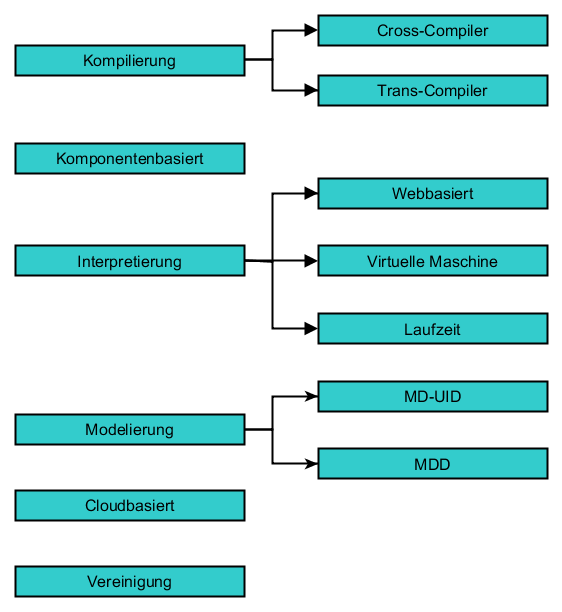
\includegraphics[width=0.8\textwidth]{Bilder/Cross_Plattform_Ansaetze}
	\caption{Haupt- und Nebenansätze zur Entwicklung von mobilen plattformübergreifenden Anwendungen}\label{graph_cross_plattform_approaches}
\end{figure}

In den folgenden Unterkapiteln werden die einzelnen Ansätze und Unteransätze näher betrachtet. Die Analyse und Betrachtung basiert auf den Informationen der Ausaurbeitung von \citep{cross_plattform_approaches}.

\subsection{Kompilierung}
Kompilierung(Compilation) ist ein Ansatz mit zwei Unterkategorien:

\begin{itemize}
	\item Cross-Compiler
	\item Trans-Compiler
\end{itemize}

Der Compiler ist ein Programm, welches den Quellcode einer High-Level Programmiersprache in einen Low-Level Code übersetzt wird. Dieser Low-Level Code ist ein Binärcode in Maschinensprache, der von dem Prozessor verstanden wird. Dieser Konvertierungsprozess wird als Kompilierung bezeichnet.

\bigskip
Man spricht von einem \textbf{Cross-Compiler}, wenn das System des Compilers unterschiedlich zu dem System ist, auf dem der kompilierte Code läuft. Die Zielsysteme können Betriebssysteme, Prozessoren oder eine Kombination aus beiden sein. Abbildung \ref{graph_compilation_XMLVM} stellt eine von XMLVM gebotene Lösung zu Cross-Compiling dar. Dies nutzt XML für die Frontend Darstellung und für die Verarbeitung des Bytecodes eine virtuelle Maschine(VM).

\begin{figure}[htbp]
	\centering
	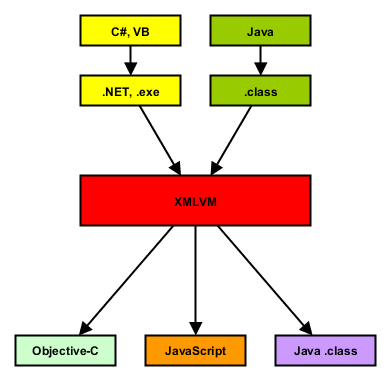
\includegraphics[width=0.7\textwidth]{Bilder/Compilation_Cross_XMLVM}
	\caption{XMLVM Prozess mit Java oder .NET Quellcode}\label{graph_compilation_XMLVM}\citep{XMLVM_Toolchain}
\end{figure}

\bigskip
Ein \textbf{Trans-Compiler} kompiliert eine High-Level Programmiersprache in eine andere High-Level Programmiersprache. Da viele Sprachen jedoch unterschiedliche Eigenschaften und Leistungsmerkmale besitzen, muss der generierte Code unter Umständen nachbearbeitet werden, wenn der Compiler diese bei der Übersetzung nicht unterstützt. Auch ist der Code durch die automatisierte Erzeugung in der Regel nur schwer lesbar. Es besteht auch eine Abhängigkeit zu regelmäßigen Updates, um die Änderungen der Quell- und Zielsysteme aktuell zu halten.

\subsection{Komponentenbasiert}
Die Komponente besteht aus einem Paket oder einem Modul, dessen Funktionen und Daten untereinander in Relation stehen. Jede Komponente besitzt eine Schnittstelle, dass die Servicedienste spezifiziert, welche von anderen Komponenten genutzt werden können. Die Kommunikation findet ausschließlich über die Schnittstellen statt, so dass eine Komponente keinerlei Informationen über den Aufbau einer anderen benötigt. 

\bigskip
Ein beispielhafter Lösungsansatz ist der \textbf{Component-Based Mobile Web Application of Cross-Plattform}. Dieser komponentenbasierte Ansatz versucht die Entwicklung mobiler Web-Apps dahingehend zu vereinfachen, dass durch das Konzept von Softwarekomponenten, die Kernfunktionalitäten modular aufgeteilt werden. Diese Module beinhalten Speichermanagement, Netzwerkkommunikation, Grafik, Dateisystem und die Systemdienstkomponenten. Dadurch erhalten die Komponenten eine Wiederverwertbarkeit und vereinfacht die Migration auf andere Plattformen. Jede Plattform kann dieselben Schnittstellen nutzen, benötigt jedoch eine eigene innere Implementierung für die Unterstützung. 

\subsection{Interpretierung}
Bei der Interpretierung übersetzt ein Interpreter (Dolmetscher) den Quellcode in ausführbare Anweisungen. Dies geschieht in Echtzeit mit Hilfe einer dedizierten Maschine. Hierbei existieren drei Unteransätze:

\begin{itemize}
	\item Virtuelle Maschine (VM)
	\item Webbasiert (Web-based)
	\item Laufzeit Interpretation (Runtime Interpretation)
\end{itemize}

Die bekannteste \textbf{virtuelle Maschine} ist die Java Virtual Machine (JVM). Diese verfügt über eine eigene komplette Hardwarearchitektur wie einer CPU, Stack, Register und ein korrespondierendes Befehlssystem. Die Grundidee hierbei ist es die mobile App mit einer plattformübergreifenden Sprache zu entwickeln, die auf der dedizierten, virtuellen Maschine läuft und auf entsprechenden Plattformen installiert ist. In Abbildung \ref{graph_interpreter_Dalvik} wird der Interpretierungsablauf der von Android bekannten Dalvik VM dargestellt.

\begin{figure}[htbp]
	\centering
	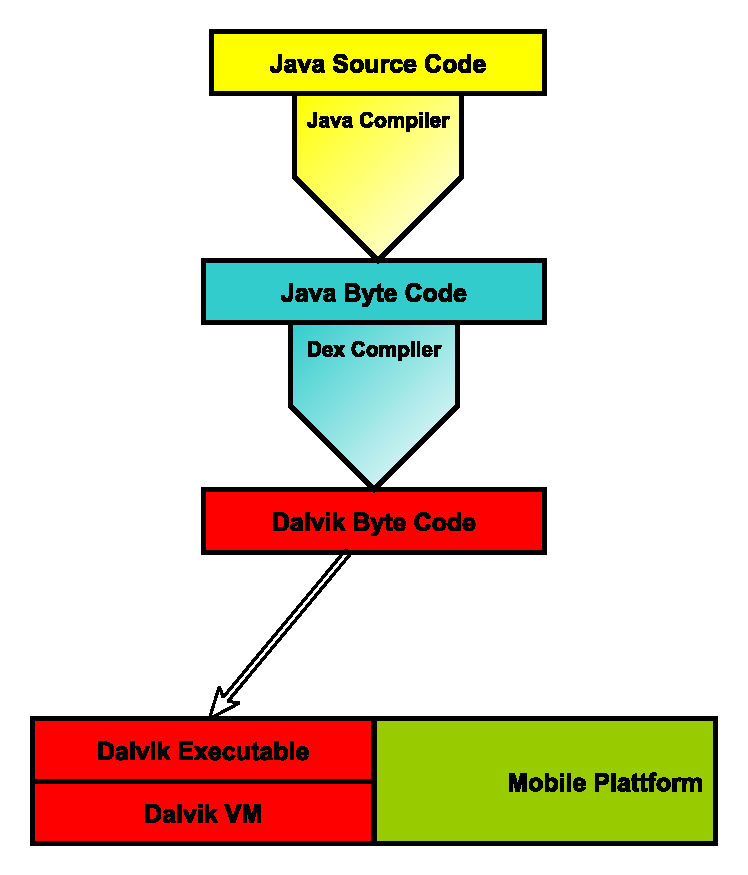
\includegraphics[width=0.6\textwidth]{Bilder/Interpretation_VM_Dalvik}
	\caption{Ablauf des Dalvik VM Interpreter}\label{graph_interpreter_Dalvik}
\end{figure}

\bigskip
\textbf{Webbasierte} Tools verwenden Technologien wie HTML(5), Javascript und CSS, die auf verschiedenen Plattformen ausführbar sind. Der Zugriff auf Hardwarekomponenten wie Kamera und Sensoren erfolgt durch Wrapper. Wrapper sind Adapter oder Schnittstellen, um auf die nativen APIs zugreifen zu können. Abbildung \ref{graph_interpreter_PhoneGap} zeigt die Kommunikation und Interpretierung des Webbasierten Interpreters PhoneGap von Adobe.

\begin{figure}[htbp]
	\centering
	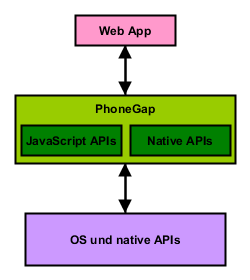
\includegraphics[width=0.5\textwidth]{Bilder/Interpretation_Web_PhoneGap}
	\caption{Vereinfachter Ablauf des PhoneGap Interpreters von Adobe}\label{graph_interpreter_PhoneGap}
\end{figure} 

\bigskip
Die \textbf{Laufzeit} ist eine Ausführungsumgebung und eine Schicht, welche die mobile App auf der nativen Plattform lauffähig macht. Bei diesem Ansatz wird der Quellcode in Bytecode umgewandelt und dann zur Laufzeit von einer virtuellen Maschine ausgeführt. In Abbildung \ref{graph_interpreter_Titanium} wird die Verarbeitung von Appcelerators Titanium-Interpreters dargestellt.

\begin{figure}[htbp]
	\centering
	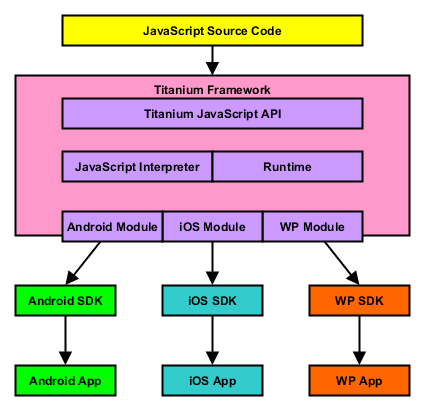
\includegraphics[width=0.7\textwidth]{Bilder/Interpretation_Runtime_Titanium}
	\caption{Ablauf des Titanium Interpreters von Appcelerator}\label{graph_interpreter_Titanium}
\end{figure}

\subsection{Modellierung}
Bei der Modellierung verwenden Entwickler abstrakte Modelle, um die Funktionen und / oder die Benutzeroberfläche der Anwendungen zu beschreiben. Diese Modelle werden für jede Zielplattform in entsprechenden Quellcode transformiert. Hierbei gibt es die Ansätze des Model-Based User Interface Development (MB-UID) und des Model-Driven Development (MDD).

\bigskip
\textbf{MB-UID} wird genutzt, um die Benutzeroberfläche durch die formale Beschreibung von Aufgaben, Daten und Benutzern einer App automatisch zu generieren. Hierbei wird zwischen der Benutzeroberfläche und der App-Logik unterschieden.
Für die Generierung existieren zwei Strategien.

\begin{itemize}
	\item Eine Generierung zur Laufzeit der App, die eine Websysteme adaptiert und basiert auf Anfrage- und Antwortprotokollen (request / response). Eingeschränkt wird dies durch die Voraussetzung einer dauerhaften Verbindung zu einem Server.
	
	\item Die Generierung während der Entwicklungszeit, also vor Ausführung der Anwendung. Hier kann der Entwickler das generierte Interface überprüfen und zu jeder Plattform spezifische Funktionalitäten hinzufügen. Dabei kann die Funktion zur Verbindungsart festgelegt werden, also ob eine dauerhafte Verbindung bestehen soll oder zu einem selbst bestimmten Zeitpunkt synchronisiert werden soll.
\end{itemize}

\bigskip
Das Hauptkonzept von \textbf{MDD} ist die Generierung von plattformspezifischen Versionen, basierend auf dem plattformunabhängigen, abstrakten Modell. Das Modell wird zum Beispiel durch Domain-Specific Language (DSL) beschrieben.

\subsection{Cloudbasiert}
In diesem Ansatz geschieht die Verarbeitung der Anwendung nicht lokal auf dem Gerät, sondern auf einem Cloudserver. Dabei werden einige Cloudeigenschaften verwendet, wie Flexibilität, Virtualisierung, Sicherheit und dynamisches Management. Die Clientanwendung ist dabei weitest möglich reduziert, da diese nur Basisprozesse benötigt. Dies wird Thin-Client genannt, da wie in Abbildung \ref{client_aufgaben} nur Ein- und Ausgabe verarbeitet werden müssen. Cloudbasierte Anwendungen sollen dadurch besonders energieeffizient sein.

\begin{figure}[htbp]
	\centering
	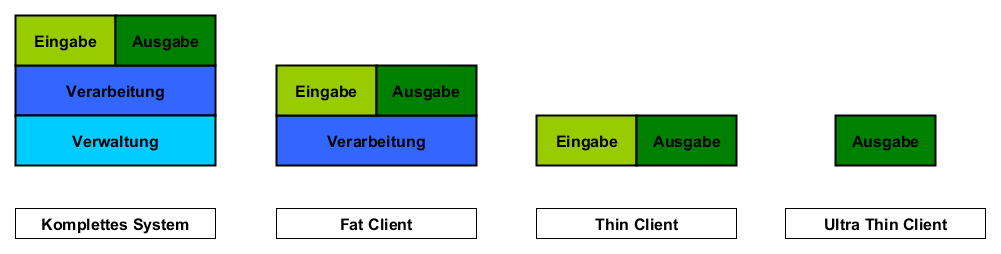
\includegraphics[width=1\textwidth]{Bilder/Aufgaben_Endgeraet}
	\caption{Aufgaben von Client-Anwendungen}\label{client_aufgaben}
\end{figure}

Da zur Zeit der Bearbeitung zu diesem Ansatz keine direkten Realisierungen gefunden worden, sondern überwiegend der theoretische Aufbau einer solchen Applikation, wird dieser Teil nicht weiter vertieft.

\subsection{Vereinigung}
Dieser Ansatz versucht die besten Eigenschaften verschiedener Ansätze zusammenzuführen, von den jeweiligen Vorteilen zu profitieren und Nachteile zu minimieren.

\bigskip
Ein \textbf{unbetitelter Lösungsansatz} vereinigt den komponentenbasierten Ansatz mit dem Cross Compiler und einer darauf angepassten Universalsprache. Um die nativen Hardwarefunktionen wie Kamera und GPS, sowie native Softwareeigenschaften wie Buttons und andere Interaktionsfelder anzusprechen, wird eine Sammlung an Komponenten erstellt. Implementierungen dieser Komponenten können durch gemeinsame Schnittstellen für jede Zielplattform erfolgen. Dieses Framework soll dem Entwickler ermöglichen, Applikationen zu entwickeln, die auf nativen Code und der Universalsprache basieren. Diese Sprache wird der App als zusätzliche Kommunikationsschicht und Schnittstelle hinzugefügt, um die Komponenten und deren Methoden anzusprechen.(Abb. \ref{graph_merge_component_based}) Der Entwickler implementiert nur eine minimale Struktur der App auf nativer Basis, welche die Benutzerschnittstelle und Navigation beinhaltet. An welcher Stelle und auf welche Weise die Komponenten integriert werden, wird durch die Universalsprache definiert. Das Framework regelt die Codeintegrierung innerhalb des nativen Codes. Bei diesem Lösungsansatz ist es erforderlich die Benutzerschnittstelle für jede Plattform manuell zu definieren. Dabei liegt der funktionale Fokus auf allgemeingültigen Funktionen, ohne Berücksichtigung der plattformspezifischen.

\begin{figure}[htbp]
	\centering
	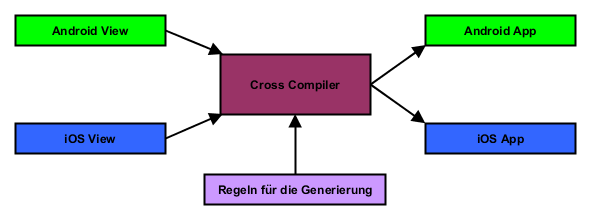
\includegraphics[width=0.9\textwidth]{Bilder/Merge_Component_based}
	\caption{Funktion eines komponentenbasierten Mergeansatz}\label{graph_merge_component_based}
\end{figure}

\bigskip
\textbf{Integrated Cross-Platform Mobile Development (ICPMD)} ist eine weitere Lösung die auf dem Merge-Prinzip aufbaut und drei Verwendungsszenarios unterstützt. Diese Szenarios sind, wie in Abbildung \ref{graph_merge_integrated_based} dargestellt, abhängig von dem gegebenen Input.

\bigskip 
Der Entwickler hat…
 
\begin{enumerate}
	\item …bereits ein bestehendes Projekt (z.B. Windows Phone) und möchte dies auf weitere Plattformen (z.B. iOS und Android) ausweiten.
	
	\item …definierte Anforderungen und möchte daraus, auf bestimmte Zielplattformen, eine mobile App erzeugen.
	
	\item …ein Projekt basierend auf dem abstrakten Modell und möchte dies aktualisieren und dann speichern oder daraus, auf bestimmte Zielplattformen, eine mobile App erzeugen.
\end{enumerate}

\begin{figure}[htbp]
	\centering
	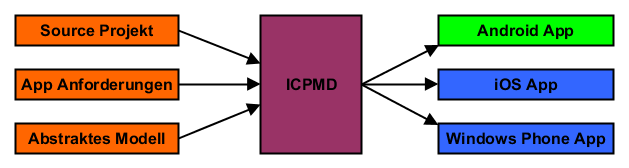
\includegraphics[width=1\textwidth]{Bilder/Merge_Integrated_based}
	\caption{Drei Szenarien bei ICPMD}\label{graph_merge_integrated_based}
\end{figure}

\section{Übersicht der Ansätze}
Tabelle \ref{table_all_approaches} fasst die vorigen Ansätze zur plattformübergreifenden Entwicklung in Kurzform zusammen, benennt die jeweiligen Vor- und Nachteile, sowie die Namen bekannter Lösungen.

\begin{table}[htbp]
	\centering
	\resizebox{\textwidth}{!}{%
		\begin{tabular}{|c|c|p{8cm}|p{6cm}|p{3,2cm}|}
			\hline
			\rowcolor[HTML]{000000} 
			{\color[HTML]{FFFFFF} \textbf{Ansatz}} & {\color[HTML]{FFFFFF} \textbf{Unteransatz}} & \multicolumn{1}{c|}{\cellcolor[HTML]{000000}{\color[HTML]{FFFFFF} \textbf{Pro}}}                                                                                                                                                                                                                                                 & \multicolumn{1}{c|}{\cellcolor[HTML]{000000}{\color[HTML]{FFFFFF} \textbf{Contra}}}                                                                                                                    & \multicolumn{1}{c|}{\cellcolor[HTML]{000000}{\color[HTML]{FFFFFF} \textbf{\begin{tabular}[c]{@{}c@{}}Beispielhafte\\ Lösungsansätze\end{tabular}}}} \\ \hline
			\textbf{Kompilierung}                  & Cross-Compiler                              & Wiederverwertung eines existierenden Quellcodes durch Cross-Kompilierung auf eine andere Plattform.Die resultierende Applikation ist native und besitzt somit die Vorteile einer nativen App.                                                                                                                                    & Die Zuordnungen zwischen zwei Sprachen ist sehr aufwendig, so dass hauptsächlich die gemeinsamen Eigenschaften berücksichtigt werden.                                                                  & MoSync, Corona, Neomades, XMLVM                                                                            \\ \hline
			\textbf{}                              & Trans-Compiler                              & Kann genutzt werden, um veraltete Applikationen und deren veralteter Code auf eine neuere Version derselben Sprache zu übersetzen. Wiederverwertung eines existierenden Quellcodes durch Trans-Kompilierung auf eine andere Plattform.Die resultierende Applikation ist native und besitzt somit die Vorteile einer nativen App. & Konzentriert sich ausschließlich auf die gemeinsamen APIs der Quell- und der Zielsprache. Benötigt regelmäßige Aktualisierungen, um die Änderungen der APIs in Quell- und Zielsprache zu unterstützen. & JUniversal                                                                                                                                    \\ \hline
			\textbf{Komponentenbasiert}            &                                             & Vereinfacht die Unterstützung neuer Plattformen durch definierte Schnittstellen bei implementierten Komponenten.                                                                                                                                                                                                                 & Konzentriert sich nur auf die Gemeinsamkeiten der unterstützten Plattformen.                                                                                                                           & Theoretisch                                                                                                                                        \\ \hline
			\textbf{Interpretation}                & Webbasiert                                  & Leicht zu erlernen und zu benutzen, da es auf bekannten Web-Technologien aufbaut.                                                                                                                                                                                                                                                & Die Benutzerschnittstelle von webbasierten Apps besitzen nicht das gleiche Aussehen und Handhabung wie bei nativen Apps. Geringere Perfomance gegenüber nativen Apps.                                  & PhoneGap, Rhomobile, xFace                                            \\ \hline
			\textbf{}                              & Virtuelle Maschine                          & Geringere Gesamtgröße und schnellerer Download der Apps, da alle benötigten Bibliotheken und Funktionen in der VM gespeichert sind.                                                                                                                                                                                              & Langsame Ausführung der Applikation auf der VM. Die VM muss erst aus einem Store geladen werden, was auf iOS nicht unterstützt wird.                                                                   & MobDSL                                                                                                                                               \\ \hline
			\textbf{}                              & Laufzeit                                    & Der Quellcode muss nur einmal geschrieben werden.                                                                                                                                                                                                                                                                                & Die Perfomance beim Laden der App ist gering, da der Interpretierungsvorgang bei jeder einzelnen Ausführung stattfindet.                                                                               & Titanium, Xamarin                                        \\ \hline
			\textbf{Modellierung}                  & MD-UID                                      & Spart Entwicklungszeit durch Generierung des UI-Codes. Nützlich für Prototyping, durch schnelle UI-Entwicklung und dadurch frühe Evaluierung der Benutzerfreundlichkeit.                                                                                                                                                         & Muss sich bei den einzelnen Plattformen auf ähnliche Benutzerschnittstellen konzentrieren.                                                                                                             &  XMobile                                                                                                                                            \\ \hline
			\textbf{}                              & MDD                                         & Die Modellierungssprache ist effektiv, um Anforderungen zu definieren. Der Fokus liegt auf der Funktionalität und nicht an der technischen Implementierung.                                                                                                                                                                      & Kann existierenden, nativen Quellcode nicht verarbeiten.                                                                                                                                               & JSAF, MD2, Jelly, AppliDE                                                                             \\ \hline
			\textbf{Cloudbasiert}                 &                                             & Verarbeitungsprozesse werden in eine Cloud ausgelagert.                                                                                                                                                                                                                                                                          & Das Endgerät und die App benötigen eine schnelle, permanente Netzwerkverbindung.                                                                                                                       &  Theoretisch                                                                                                                                         \\ \hline
			\textbf{Vereinigung}                   &                                             & Vorteile aus den Stärken anderer Ansätze. Bietet dem Entwickler vielseitige Möglichkeiten.                                                                                                                                                                                                                                       & Benötigt hohen Entwicklungsaufwand.                                                                                                                                                                    &  ICPMD                                                                                                                                             \\ \hline
		\end{tabular}
	}
	\caption{Übersicht aller Ansätze}
	\label{table_all_approaches}
\end{table}

\section{Plattformübergreifende Entwicklung mobiler Applikationen ohne den Schwerpunkt Spieleentwicklung}
Plattformübergreifende Entwicklung für mobile Plattformen ist nicht nur für die Spieleentwicklung interessant.
In der Thesis „\textit{Plattformabhängige und –unabhängige Entwicklung mobiler Anwendungen am Beispiel von Geo-Wikipedia-App}“ \citep{cross_plattform_development_vehse} wird ebenfalls die plattformübergreifende Entwicklung analysiert, jedoch liegt hier nicht der Fokus auf Game-spezifischen Applikationen und Entwicklungswerkzeugen. Hier wird in Kapitel 2.2 auch auf die verschiedenen Herangehensweisen eingegangen und deren Resultate klassifiziert. Weiterhin wird eine Auswahl der bekannteren Cross-Plattform Entwicklungstools (PhoneGap, Xamarin, Appcelerator) analysiert. Im Gegensatz zu der Arbeit von Benjamin Vehse, setzt diese Thesis den Schwerpunkt auf Frameworks und Engines zur Spieleentwicklung und geht von daher nicht weiter auf die genannten und vorangegangenen Entwicklungswerkzeuge ein.


%TODO: Kapitel 5
\chapter{Plattformübergreifende Spieleentwicklung}
\section{Anforderungen für vergleichbare Entwicklungstools}
\section{Gamespezifische Frameworks und Engines}
\subsection{libGDX}
\subsection{Cocos2D-X}
\subsection{Unity3D}
\subsection{Weitere Frameworks}
%Eigenheiten, Cross Plattform Ansatz, RoboVM

%TODO: Kapitel 6
\chapter{Analyse der Frameworks}
%Features und Einschränkungen

\section{Zielplattformen}
Die Menge an Zielplattformen unterscheidet sich in den Bereichen Mobil, Destop und Web nur geringfügig. In Tabelle \ref{zielplattformen_frameworks} wird deutlich, dass sich die Menge an unterstützten Plattformen in diesen Kategorien, bei Cocos2D-x und Unity3D kaum unterscheidet. Das Blackberry OS wurde von beiden, hauptsächlich mangels Nachfrage, aus dem Programm genommen. Einzig libGDX stellt noch die Möglichkeit, Spiele hierfür zu entwickeln. Dafür befinden sich in dem Katalog von libGDX die meisten Lücken, wovon die gravierendste, aber derzeit noch verzeihbare, das Fehlen von Windows Phone und Universal Windows ist. Dennoch bieten alle drei Frameworks die Möglichkeit, gleichzeitige Entwicklung bei iOS und Android, als die wichtigsten mobilen Plattformen zuzulassen. 

\begin{table}[htbp]
	\centering
	\resizebox{0.8\textwidth}{!}{%
		\begin{tabular}{cccc}
			\rowcolor[HTML]{000000} 
			\cellcolor[HTML]{FFFFFF}{\color[HTML]{000000} \textbf{}} & {\color[HTML]{FFFFFF} \textbf{Cocos2D-X}} & {\color[HTML]{FFFFFF} \textbf{LibGDX}} & {\color[HTML]{FFFFFF} \textbf{Unity3D}} \\
			\cellcolor[HTML]{000000}{\color[HTML]{FFFFFF} Mobil}           &                                         &                                        &                                         \\
			\cellcolor[HTML]{C0C0C0}iOS                                             & {\color[HTML]{000000} X}                & {\color[HTML]{000000} X}               & {\color[HTML]{000000} X}                \\
			\cellcolor[HTML]{C0C0C0}Android                                         & {\color[HTML]{000000} X}                & {\color[HTML]{000000} X}               & {\color[HTML]{000000} X}                \\
			\cellcolor[HTML]{C0C0C0}Windows Phone 8                                 & {\color[HTML]{000000} X}                & {\color[HTML]{000000} }                & {\color[HTML]{000000} X}                \\
			\cellcolor[HTML]{C0C0C0}Tizen                                           & {\color[HTML]{000000} X}                & {\color[HTML]{000000} }                & {\color[HTML]{000000} X}                \\
			\cellcolor[HTML]{C0C0C0}Blackberry                                      & {\color[HTML]{000000} }                 & {\color[HTML]{000000} X}               & {\color[HTML]{000000} }                 \\
			& {\color[HTML]{000000} }                 & {\color[HTML]{000000} }                & {\color[HTML]{000000} }                 \\
			\cellcolor[HTML]{000000}{\color[HTML]{FFFFFF} Desktop}         & {\color[HTML]{000000} }                 & {\color[HTML]{000000} }                & {\color[HTML]{000000} }                 \\
			\cellcolor[HTML]{C0C0C0}Mac                                             & {\color[HTML]{000000} X}                & {\color[HTML]{000000} X}               & {\color[HTML]{000000} X}                \\
			\cellcolor[HTML]{C0C0C0}Windows                                         & {\color[HTML]{000000} X}                & {\color[HTML]{000000} X}               & {\color[HTML]{000000} X}                \\
			\cellcolor[HTML]{C0C0C0}Universal Windows Platform                      & {\color[HTML]{000000} X}                & {\color[HTML]{000000} }                & {\color[HTML]{000000} X}                \\
			\cellcolor[HTML]{C0C0C0}Linux / Steam OS                                & {\color[HTML]{000000} X}                & {\color[HTML]{000000} X}               & {\color[HTML]{000000} X}                \\
			& {\color[HTML]{000000} }                 & {\color[HTML]{000000} }                & {\color[HTML]{000000} }                 \\
			\cellcolor[HTML]{000000}{\color[HTML]{FFFFFF} Web}             & {\color[HTML]{000000} }                 & {\color[HTML]{000000} }                & {\color[HTML]{000000} }                 \\
			\cellcolor[HTML]{C0C0C0}Web GL                                          & {\color[HTML]{000000} X}                & {\color[HTML]{000000} X}               & {\color[HTML]{000000} X}                \\
			\cellcolor[HTML]{C0C0C0}Web Player                                      & {\color[HTML]{000000} }                 & {\color[HTML]{000000} }                & {\color[HTML]{000000} X}                \\
			\cellcolor[HTML]{C0C0C0}Java Applet                                     & {\color[HTML]{000000} }                 & {\color[HTML]{000000} X}               & {\color[HTML]{000000} }                 \\
			& {\color[HTML]{000000} }                 & {\color[HTML]{000000} }                & {\color[HTML]{000000} }                 \\
			\cellcolor[HTML]{000000}{\color[HTML]{FFFFFF} \textbf{Gesamt}}             & {\cellcolor[HTML]{BEBEBE} 9}                 & {\cellcolor[HTML]{BEBEBE} 8}                & {\cellcolor[HTML]{BEBEBE} 10}                 \\
		\end{tabular}
	}
	\caption{Unterstützte Zielplattformen der Frameworks}
	\label{zielplattformen_frameworks}\citep{unity_public_relations,cocos2d_main_features,libGDX_main_features}
\end{table}

\section{Programmiersprachen}
Die gewählten Spieleframeworks unterscheiden sich bei den verfügbaren Programmiersprachen komplett untereinander. Das verschafft Entwicklern mit unterschiedlichen Kenntnissen, einen leichteren Einstieg in die Spieleentwicklung, durch die Wahl einer vertrauten Sprache. Da manche Frameworks auch mehr als eine Sprache unterstützen, werden diese zugunsten der Übersichtlichkeit in eigenen Unterkapiteln behandelt.

\subsection{libGDX}
\label{subsec:libGDX}
\textbf{libGDX} nutzt einzig und allein Java für die Entwicklung, was für reine Android Spiele ein großer Vorteil ist. Denn dadurch werden bei der Kompilierung kaum Kompromisse eingegangen.
Java ist eine weitverbreitete, objektorientierte Programmiersprache, die erstmalig 1995 von dem Unternehmen Sun Microsystem vorgestellt wurde. 2010 übernahm das Unternehmen Oracle Sun Microsystem und die Weiterentwicklung von Java. Es entstanden verschiedene spezialisierte Technologielösungen. Die bekanntesten und meistgenutzten stellen dabei Java SE (Standard Edition) und Java EE (Enterprise Edition) dar. Java SE beinhaltet die komplette Standardbibliothek, wobei Java EE um Bibliotheken für die Entwicklung von Server-, Netzwerk- und Webanwendungen erweitert wurde. Das derzeit aktuelle JDK 8 soll 2016 auf Version 9 aufsteigen. \citep{java_9}
Die Sprache gilt als plattformübergreifend, da Programme in einer virtuelle Maschine ausgeführt werden, der JVM(Java Virtual Machine). Diese führt den bei der Kompilierung erstellten Bytecode aus und prüft das Programm auf Laufzeitfehler. 
Die Syntax lehnt sich an C++ und C. Die Typisierung ist statisch und gilt allgemein als sicher im Speicherbereich. \citep{java_kompakt}

\subsection{Cocos2D-X}
Mit \textbf{Coco2D-X} hat man die Wahl zwischen C++, Lua und JavaScript, welche auf allen unterstützten Plattformen funktionieren. Einzige Einschränkung liegt bei JavaScript, da diese sich bei Cocos2D-X nicht mit Windows Phone verknüpfen lässt. \citep{cocos2d_main_features}

\bigskip
Lua ist eine schnelle, von der Syntax simpel gehaltene Skriptsprache, mit objektorientierten Eigenschaften. Die geschriebenen Skripte werden durch einen Interpreter in Bytecode übersetzt und ist kompatibel mit der Sprache C. Lua befindet sich derzeit in Version 5.3 und wird häufig in der Spieleentwicklung eingesetzt. \citep{lua_about}

\bigskip
Mit der Unterstützung von C++, welches direkt von C abgeleitet ist, hat man die Möglichkeit äußerst performante und portable Software zu schreiben. Voraussetzung ist dabei ein sicherer Umgang, da C++ im Vergleich mit anderen High-Level Sprachen, sich weniger um Logikfehler kümmert und entsprechend auch keine Warnungen ausgibt. Die aktuelle Version ist C++14.

\bigskip
Für Entwickler die beispielsweise Erfahrungen im Webbereich besitzen, bietet die Verwendung von JavaScript einen weiteren Einstieg in Cocos2D-X.
JavaScript ist eine Skriptsprache die es seit 1995 gibt und für dynamisches HTML in Webbrowsern entwickelt wurde. Trotz der Namensähnlichkeit zu Java, unterscheiden sich die beiden Sprachen grundlegend voneinander. JavaScript wird in der Regel genutzt um Client-seitige Logik innerhalb von HTML Dokumenten zu ermöglichen. Mit der Programmiersprache Java hingegen, können eigenständige Anwendungen aufgebaut werden. Die Sprache folgt Spezifikationen der privaten Normungsorganisation ECMA (European Computer Manufacturers Association), die Standardisierungen von Informationstechnologien entwickelt, die Richtigkeit deren Verwendung fördert und eine frei zugängliche Veröffentlichung dazu liefert. Der standardisierte Kern von JavaScript, wird als ECMAScript (ECMA 262) bezeichnet und beschreibt eine dynamische Typisierung, mit objektorientierten, aber klassenlosen Eigenschaften. Objekte basieren auf sogenannten Prototypen, die als Funktionen beschrieben werden. Nach der Instanziierung ist es möglich, das Objekt um zusätzliche Eigenschaften zu erweitern. Skripte können imperativ, aber auch funktional aufgebaut werden. Geschriebene Skripte werden durch einen Interpreter übersetzt. Basierend auf JavaScript, entstanden viele Bibliotheken und Frameworks, um beispielsweise serverseitige Netzwerkanwendungen zu betreiben (Node.js) oder Entwurfsmuster aus der Softwareentwicklung zu nutzen (Angular.js).
ECMAScript befindet sich seit 2015 in Version 6. \citep{learning_javascript}

\subsection{Unity3D}
In \textbf{Unity3D} finden die Sprachen C\#, UnityScript und Boo Verwendung. Alle für Unity3D nutzbaren Sprachen entspringen Microsofts .NET Framework. Das bedeutet auch, dass es möglich ist weitere .NET Sprachen zu benutzen, wenn diese ihre Skripte in das DLL (Dynamically Linked Library) Format kompilieren können. Diese DLL Dateien können dann dem Unity Projekt hinzugefügt und verwendet werden. \citep{unity_managed_plugins}

\bigskip
Boo ist eine von Python beeinflusste Sprache für .NET und Mono, welche ohne Klammern und Semikolons auskommt. Die Typisierung ist generell statisch, kann aber trotzdem dynamische \textit{Duck-Typing} Eigenschaften nutzen. \citep{boo_about} Der Name Duck-Typing entsprang dem sogenannten \textit{Ententest} zur Typisierung, welcher wiederum auf einem Gedicht von James Whitcomb Riley zurückzuführen ist.

\bigskip
“\emph{When I see a bird that walks like a duck and swims like a duck and quacks like a duck, I call that bird a duck.}” \citep{ducktest}

\bigskip
Beim Duck-Typing werden Objekte nicht durch ihre Klasse typisiert, sondern durch die vorhandenen Attribute und Methoden. Daher findet die Typisierung erst zur Laufzeit durch den Interpreter statt. Aufgrund des seltenen Gebrauchs, wird Boo seit Unity 5.0 in der Dokumentation nicht mehr unterstützt.

\bigskip
Oft wird UnityScript in der Unity Community, aber auch von dem Unternehmen selbst, fälschlicherweise mit JavaScript gleichgesetzt, als wären die beiden Sprachen äquivalent. Auch wenn syntaktische Ähnlichkeiten bestehen, gibt es große semantische Unterschiede.
UnityScript kann, wie die meisten objektorientierten Programmiersprachen, Klassen definieren und daraus Objekte erstellen. JavaScript hingegen besitzt zwar ebenfalls objektorientierte Eigenschaften, wobei diese anstatt Klassen aber sogenannte Prototypes verwendet. Des Weiteren kann UnityScript im Gegensatz zu JavaScript, Klassen, Objekte, Funktionen und Variablen mit Zugriffsmodifikatoren/Sichtbarkeiten versehen. UnityScript wurde speziell für die Unity3D Engine konzipiert und ist proprietär, was es schwierig macht, genaue Spezifikationen zu finden. \citep{unity_unityscript_vs_javascript}

\bigskip
C\# oder auch Visual C\# ist eine von Microsoft entwickelte Programmiersprache, die durch ECMA-334 standardisiert ist und sich aktuell in Version 6.0 befindet. Die Standardisierung bezieht sich allerdings nur auf die Sprache selbst und nicht auf Programme die in Verbindung mit dem .NET Framework realisiert worden. Alternativ zu .NET bietet Mono ein Open Source Framework inklusive Compiler für C\# an. Die Syntax der objektorientierten Sprache weißt große Ähnlichkeiten mit Java auf und wird oft mit dieser verglichen. Die Typisierung ist grundsätzlich statisch, wobei optional auch dynamische Typen genutzt werden können. \citep{csharp_in_depth}
Laut Statistik, sind etwa 80\% der Unity Projekte in C\# geschrieben. \citep{unity_languages}

\section{Entwicklungsumgebungen}
Für den Prozess der Entwicklung besteht bei jedem Framework die Wahlmöglichkeit zwischen mehreren IDEs. Praktisch kann selbstverständlich jeder textbasierte Editor zur Programmierung verwendet werden, aber um den Komfort von passendem Code-Highlighting und die direkte Projekterstellung zu nutzen, empfiehlt es sich die unterstützten Entwicklungsumgebungen zu verwenden. Diese stehen bei den drei vorgestellten Spieleframeworks in direkter Abhängigkeit zu dem verwendeten Betriebssystem.

\subsection{Systembedingte Einschränkungen}
Es gilt für jedwede Erzeugung von iOS Applikationen, das die Apple IDE Xcode unumgänglich ist. Diese ist auch ausschließlich unter OS X Systemen erhältlich und einsetzbar. Um die iOS Applikation testen zu können, benötigt man seit Xcode 7 nur noch eine gültige Apple ID. Um die App zu veröffentlichen, ist man letztlich aber dennoch verpflichtet eine Mitgliedschaft des Apple Developer Program zu erwerben. Diese geht mit aktuellen 99 US Dollar jährlich einher. In der Mitgliedschaft sind die Rechte zur Veröffentlichung von iOS, watchOS und OS X Anwendungen, sowie das Anlegen und Durchführen von Beta-Tests mit Testflight und diverse andere Features. \citep{apple_developer_program}

\bigskip
Um iOS Apps mit libGDX zu erstellen, ist man zudem an einen speziellen Kompilierer gebunden, der Java in Obective-C Code übersetzen kann. Hierfür wird mit RoboVM zusammengearbeitet. Die Einbindung dieses Tools ist beispielsweise in Eclipse oder in auf Intellij IDEA basierten Entwicklungsumgebungen möglich. Eine eigene IDE mit Namen RoboVM Studio steht ebenfalls zur Wahl. Für die Nutzung von RoboVM fallen im Normalfall kosten ab derzeit 25 US Dollar für eine Einzellizenz an. Es werden jedoch auch reduzierte bis kostenfreie Modelle für Indie Entwickler oder Studenten angeboten. \citep{roboVM}

\bigskip
Die Erstellung von Windows Phone Apps ist mit der Verwendung von Visual Studio verbunden. Diese benötigt mindestens Windows 7. Um den Simulator nutzen zu können, wird Microsofts Virtualisierungstechnik Hyper-V vorausgesetzt, wofür eine Windows 8 Pro oder Windows 10 Pro Version notwendig ist. \citep{visual_studio}

\subsection{Unterstützte IDEs}
In Tabelle \ref{ides} werden die Editoren aufgelistet, die für die Bearbeitung des Quellcodes unterstützt und empfohlen werden. Abhängig welche Programmiersprache man bevorzugt, hat man pro Gameframework eine oder mehrere IDEs zur Auswahl. Wie im vorigen Kapitel bereits erwähnt, ist für jede iOS App Xcode unter OS X verpflichtend, ebenso wie Visual Studio für Windows Phone Anwendungen. Daher werden diese nicht zusätzlich für jedes Framework markiert. Die jeweiligen Vor- und Nachteile der einzelnen Entwicklungsumgebungen werden in dieser Arbeit nicht weiter behandelt und dieser Teil soll auch nicht weiter vertieft werden. Es dient lediglich der Vollständigkeit.

\begin{table}[htbp]
	\centering
	\resizebox{\textwidth}{!}{%
		\begin{tabular}{cccccc}
			\rowcolor[HTML]{000000} 
			{\color[HTML]{FFFFFF} \textbf{IDE}}            & {\color[HTML]{FFFFFF} \textbf{Betriebssystem}} & {\color[HTML]{FFFFFF} \textbf{Sprache}} & {\color[HTML]{FFFFFF} \textbf{libGDX}} & {\color[HTML]{FFFFFF} \textbf{Cocos2D-X}} & {\color[HTML]{FFFFFF} \textbf{Unity3D}} \\
			{\color[HTML]{000000} \textbf{Eclipse}}        & {\color[HTML]{000000} Windows / OS X}          & {\color[HTML]{000000} Java}                        & {\color[HTML]{000000} X}               & {\color[HTML]{000000} }                   & {\color[HTML]{000000} }                 \\
			\rowcolor[HTML]{C0C0C0} 
			{\color[HTML]{000000} \textbf{IDEA}}           & {\color[HTML]{000000} Windows / OS X}          & {\color[HTML]{000000} Java}                        & {\color[HTML]{000000} X}               & {\color[HTML]{000000} }                   & {\color[HTML]{000000} }                 \\
			{\color[HTML]{000000} \textbf{Android Studio}} & {\color[HTML]{000000} Windows / OS X}          & {\color[HTML]{000000} Java}                        & {\color[HTML]{000000} X}               & {\color[HTML]{000000} }                   & {\color[HTML]{000000} }                 \\
			\rowcolor[HTML]{C0C0C0} 
			{\color[HTML]{000000} \textbf{NetBeans}}       & {\color[HTML]{000000} Windows / OS X}          & {\color[HTML]{000000} Java}                        & {\color[HTML]{000000} X}               & {\color[HTML]{000000} }                   & {\color[HTML]{000000} }                 \\
			{\color[HTML]{000000} \textbf{RoboVM Studio}}  & {\color[HTML]{000000} Windows / OS X}          & {\color[HTML]{000000} Java}                        & {\color[HTML]{000000} X}               & {\color[HTML]{000000} }                   & {\color[HTML]{000000} }                 \\
			\rowcolor[HTML]{C0C0C0} 
			{\color[HTML]{000000} \textbf{Xcode}}          & {\color[HTML]{000000} OS X}                    & {\color[HTML]{000000} C++}                         & {\color[HTML]{000000} }                & {\color[HTML]{000000} X}                  & {\color[HTML]{000000} }                 \\
			{\color[HTML]{000000} \textbf{Cocos Code}}     & {\color[HTML]{000000} Windows / OS X}          & {\color[HTML]{000000} JavaScript / Lua}            & {\color[HTML]{000000} }                & {\color[HTML]{000000} X}                  & {\color[HTML]{000000} }                 \\
			\rowcolor[HTML]{C0C0C0} 
			\textbf{Visual Studio}                         & Windows                                        & C\# / C++                                          &                                        & X                                         & X                                       \\
			\textbf{MonoDevelop}                           & Windows / OS X                                 & C\# / UnityScript                                  &                                        &                                           & X                                      
		\end{tabular}
	}
	\caption{Unterstützte Entwicklungsumgebungen zur Bearbeitung der Codebasis} \citep{libGDX_wiki, cocos2d_main_features, unity_code_editor}
	\label{ides}
\end{table}

\section{Native Gerätefunktionen und Schnittstellen}
Smartphones und Tablets besitzen in der Regel kaum oder gar keine Hardwarebuttons, die für Anwendungen neu belegbar sind. Spiele die für solche mobilen Systeme entworfen worden, greifen daher auf eine oder zwei der beiden populärsten Steuerungsmechanismen zurück.

\bigskip
Überwiegende Praxis ist es, den vorhandenen Touchscreen für Eingaben und Interaktionen zu nutzen. Dies kann über bekannte Gesten geschehen oder über die Virtualisierung von Aktionsflächen, wie zum Beispiel Buttons und Regler. Alle drei Frameworks verfügen über Möglichkeiten, verschiedene Touchgesten zu unterscheiden.
Eine andere Möglichkeit in das Spielgeschehen einzugreifen, bieten die geräteseitigen Hardwaresensoren. Ein Anwendungsbeispiel für den Gyroskop Sensor, wäre bei Rennspielen die Simulierung eines Lenkrades, bei dem durch die Neigung des Gerätes gesteuert wird. Weiterhin gehören Accelerometer, GPS und sowohl eine Kamera zu den üblichen Gerätefunktionen.

\bigskip
\textbf{Unity3D} liefert für fast alle gängigen Gerätefunktionen entsprechende Schnittstellen, um diese zu nutzen oder mit Funktionen zu hinterlegen. Bei \textbf{libGDX} kann man auf die meisten Sensorentypen zugreifen, muss aber auf Kamera und GPS verzichten.
Hingegen kann \textbf{Cocos2D-X} bisher nur den Accelerometer ansteuern, wenn dieser vorhanden ist. Gyroskop, Kamera, GPS Lokalisierung und weiteres werden derzeit nicht unterstützt. Dadurch dass die beiden Frameworks quelloffen sind, ist bei Bedarf eine eigene Implementation theoretisch dennoch möglich. Eine offizielle Erweiterung ist demnach auch abhängig von dem Streben der Entwickler-Community. 
In Tabelle \ref{tab_schnittstellen} werden die häufigsten Gerätefunktionen und die Unterstützung durch eine Schnittstelle, der einzelnen Frameworks gelistet. 
Der Vollständigkeit halber ist zu dem Punkt Netzwerkverbindung zu sagen, dass keines der drei Frameworks ein WLAN Modul oder mobiles Internet ein- und ausschalten kann. Aus Gründen der Sicherheit, kann dies nur der Nutzer selbst. Es kann lediglich getestet werden, ob eine aktive Verbindung existiert. Für die Prüfung einer Bluetooth Verbindung, gibt es derzeit für keines eine offizielle Schnittstelle. Wenn ein Projekt die Anforderung einer bestimmten Schnittstelle besitzt, die aber in dem gewählten Framework nicht vorhanden ist, hat man dennoch die Möglichkeit diese plattformabhängig zu implementieren.

\begin{table}[htbp]
	\centering
	\resizebox{\textwidth}{!}{%
		\begin{tabular}{
				>{\columncolor[HTML]{C0C0C0}}c ccc}
			\cellcolor[HTML]{000000}{\color[HTML]{FFFFFF} \textbf{Schnittstelle}} & \cellcolor[HTML]{000000}{\color[HTML]{FFFFFF} \textbf{libGDX}} & \cellcolor[HTML]{000000}{\color[HTML]{FFFFFF} \textbf{Cocos2D-X}} & \cellcolor[HTML]{000000}{\color[HTML]{FFFFFF} \textbf{Unity3D}} \\
			Touchgesten                                                         & X                                                              & X                                                                 & X                                                               \\
			Netzwerkverbindung                                                    & X                                                               & X                                                                   & X                                                               \\
			Accelerometer                                                         & X                                                              & X                                                                 & X                                                               \\
			Gyroskop                                                              & X                                                              &                                                                   & X                                                               \\
			Vibration                                                             & X                                                              &                                                                   & X                                                              \\
			Kompass                                                               & X                                                              &                                                                   & X                                                               \\
			Kamera                                                                &                                                                &                                                                   & X                                                               \\
			Geoposition                                                           &                                                                &                                                                   & X                                                               \\
			Bluetooth                                                             &                                                                &                                                                   &                                                                 \\
		\end{tabular}
	}
	\caption{Verfügbare Schnittstellen zu den Gerätefunktionen}
	\label{tab_schnittstellen}\citep{libGDX_docs,cocos2d_docs,unity_docs}
\end{table}


\section{Game Services}
Um die Motivation und die Wiederspielbarkeit zu erhöhen, sowie neue Inhalte zur Verfügung zu stellen, können verschiedene Funktionalitäten eingebunden werden. 
Ein Erfolgssystem basiert auf dem Belohnungsprinzip und kann den Benutzer auf unterschiedliche Weise in seinem Spielverhalten motivieren. Durch definierte Herausforderungen werden verschiedene Aufgaben gestellt, wobei dem Spieler durch das Erreichen dieser, ein visuelles Feedback gegeben werden kann. Das kann beispielsweise in Form von Medaillen, Erhöhung des Spielerlevels oder einer Prozessleiste auftreten. Kompetitive Elemente können mit Bestenlisten erzielt werden, in denen bestimmte Metriken von den Spielern sortiert aufgelistet werden können. Ranglisten über die höchste Punktzahl oder die längste Spielzeit geben Anreiz sich mit anderen zu messen. 
In rundenbasierten und Echtzeit Mehrspielermodi treten zwei oder mehr Spieler gegeneinander an, um in einem Wettbewerb den besten Spieler zu ermitteln. Eine andere beliebte Variante sind Modi, in denen die Teilnehmer kooperieren, um Spielziele gemeinsam zu erreichen oder einfach unterhaltsame Erfahrungen zu schaffen.
Um verbesserungswürdige Schwachstellen in der Anwendung zu ermitteln und das Verhalten von Spielern zu messen, werden Analysesysteme verwendet. Diese ermöglichen Einblicke auf Aktivitäten und Fortschritte der Spieler und Informationen zu getätigten Käufen. Auch wie häufig ein Benutzer die Anwendung gebraucht kann gemessen werden. Diese Statistiken verhelfen zu einem besseren Verständnis der eigenen Anwendung.
Für den Erwerb von zusätzlichen, applikationsinternen Inhalten und die Abwicklung von Zahlungen sind Shop Systeme notwendig. Dies wird bei plattformübergreifenden Applikationen durch die Implementierung einer Bibliothek ermöglicht, die zu den gewünschten Zielplattformen und deren Stores, passende Schnittstellen bereitstellt. 
In Tabelle \ref{tab_game_services} werden APIs aufgelistet, die populäre Game Services in den Frameworks unterstützen. Die Tabelle zeigt ausschließlich APIs, die plattformübergreifende Eigenschaften aufweisen und auf den beiden wichtigsten, mobilen Zielplattformen iOS und Android funktionieren.

\begin{table}[htbp]
	\centering
	\resizebox{\textwidth}{!}{%
		\begin{tabular}{cccc}
			\rowcolor[HTML]{000000} 
			{\color[HTML]{FFFFFF} \textbf{Game Service}}                                                               & {\color[HTML]{FFFFFF} \textbf{libGDX}}                                            & {\color[HTML]{FFFFFF} \textbf{Cocos2D-X}}                                         & {\color[HTML]{FFFFFF} \textbf{Unity3D}}                                           \\
			\rowcolor[HTML]{C0C0C0} 
			{\color[HTML]{000000} \textbf{Erfolge}}                                                                    & \begin{tabular}[c]{@{}c@{}}Play Game Services \\ App42\end{tabular}             & \begin{tabular}[c]{@{}c@{}}Play Game Services \\ App42\end{tabular}             & \begin{tabular}[c]{@{}c@{}}Play Game Services \\ App42\end{tabular}             \\
			\cellcolor[HTML]{FFFFFF}{\color[HTML]{000000} \textbf{Bestenlisten}}                                       & \begin{tabular}[c]{@{}c@{}}Play Game Services \\ App42\end{tabular}             & \begin{tabular}[c]{@{}c@{}}Play Game Services \\ App42\end{tabular}             & \begin{tabular}[c]{@{}c@{}}Play Services \\ App42\end{tabular}             \\
			\rowcolor[HTML]{C0C0C0} 
			{\color[HTML]{000000} \textbf{Multiplayer}}                                                                & \begin{tabular}[c]{@{}c@{}}Play Game Services \\ App42 \\ Nextpeer\end{tabular} & \begin{tabular}[c]{@{}c@{}}Play Game Services \\ App42 \\ Nextpeer\end{tabular} & \begin{tabular}[c]{@{}c@{}}Play Game Services \\ App42 \\ Nextpeer\end{tabular} \\
			\cellcolor[HTML]{FFFFFF}{\color[HTML]{000000} \textbf{Spielstand sichern}}                                 & \begin{tabular}[c]{@{}c@{}}Play Game Services \\ App42\end{tabular}             & \begin{tabular}[c]{@{}c@{}}Play Game Services \\ App42\end{tabular}             & \begin{tabular}[c]{@{}c@{}}Play Game Services \\ App42\end{tabular}             \\
			\rowcolor[HTML]{C0C0C0} 
			{\color[HTML]{000000} \textbf{Analyse}}                                                                    & App42                                                                             & App42                                                                             & \begin{tabular}[c]{@{}c@{}}Unity Analytics \\ App42 \\ Soomla\end{tabular}        \\
			\cellcolor[HTML]{FFFFFF}{\color[HTML]{000000} \textbf{Shop System}}                                        & gdx-pay                                                                           & SDKBOX-IAP                                                                        & Soomla                                                                            \\
			\rowcolor[HTML]{C0C0C0} 
			{\color[HTML]{000000} \textbf{\begin{tabular}[c]{@{}c@{}}Soziale Netzwerke \\ Freundesliste\end{tabular}}} & \begin{tabular}[c]{@{}c@{}}App42 \\ Nextpeer\end{tabular}                         & \begin{tabular}[c]{@{}c@{}}App42 \\ Nextpeer\end{tabular}                         & \begin{tabular}[c]{@{}c@{}}Social API \\ App42 \\ Nextpeer \\ Soomla\end{tabular}
		\end{tabular}
	}
	\caption{Game Services und plattformübergreifende Schnittstellen}
	\label{tab_game_services}
\end{table}

\bigskip
\textbf{Play Game Services} \\
Das Framework von Google bietet zahlreiche Services für den mobilen Gaming-Bereich. Es werden die meisten in der Tabelle genannten Services für die plattformübergreifende Entwicklung unterstützt. Die Voraussetzung für den Spieler, um diese Features nutzen zu können, ist ein Account in dem Netzwerk Google+. Play Game Services bietet auch Services zur Analyse des Spielerverhaltens, jedoch sind die Angaben von Google und den Spieleentwicklungstools bezüglich der Unterstützung nicht eindeutig. Die Cloud Dienste von Google sind ohne Kosten implementierbar. \citep{play_game_services}

\bigskip
\textbf{App42} \\
App42 von ShepHertz Technologies bietet ein umfangreiches Angebot an Cloud Diensten, welches für Indie-Entwickler größtenteils kostenfrei zur Verfügung steht. Es gibt Schnittstellen für eine Vielzahl an Plattformen und Frameworks, sowohl im nativen, als auch im plattformübergreifenden Bereich. Die wichtigsten Game Services werden alle unterstützt. \citep{app42}

\bigskip
\textbf{NextPeer} \\
NextPeer bietet für die drei Game Frameworks APIs für die Unterstützung von Multiplayer Spielen und Anbindungen an soziale Netzwerke. Für die Nutzung steht ebenfalls eine kostenfreie Variante zur Auswahl. \citep{nextpeer}


\section{Produktvarianten}
Das Java Framework \textbf{libGDX} ist das offizielle Kernprojekt. Eigene Varianten sind durchaus möglich, aber derzeit sind keine weiteren populären Ableger bekannt. Die Community konzentriert sich demnach hauptsächlich auf die Weiterentwicklung der Hauptversion oder auf eigene Erweiterungen in Form von Plugins.

\bigskip
\textbf{Cocos2D-X} ist eine von mehreren Abzweigungen aus der Cocos2D Familie. Stamm der Entwicklung bildet das mit Python entwickelte Cocos2D, welches selbige Sprache auch für die Entwicklung daraus resultierender Desktopanwendungen benutzt. Der erste daraus abgeleitete Ableger Cocos2D-iPhone oder auch bekannt als Cocos2D-ObjC, erlaubt die Implementierung auf mobile Apple Geräte. Diese können mit den plattformüblichen nativen Sprachen Objective-C und Swift konstruiert werden. Aus dieser Version entsprangen direkt wiederum viele weitere Varianten für gezielte Sprachen und Anwendungen, als auch das in dieser Arbeit behandelte Cocos2D-X für die Unterstützung multipler Plattformen. Die Cocos2D Frameworks iPhone, X, HTML5 und dem Editor SpriteBuilder sind kooperierende Projekte und folgen demselben Leitplan. Daher haben sie ein koordiniertes Updateverhalten. \citep{cocos2d_relationships}

\begin{figure}[htbp]
	\centering
	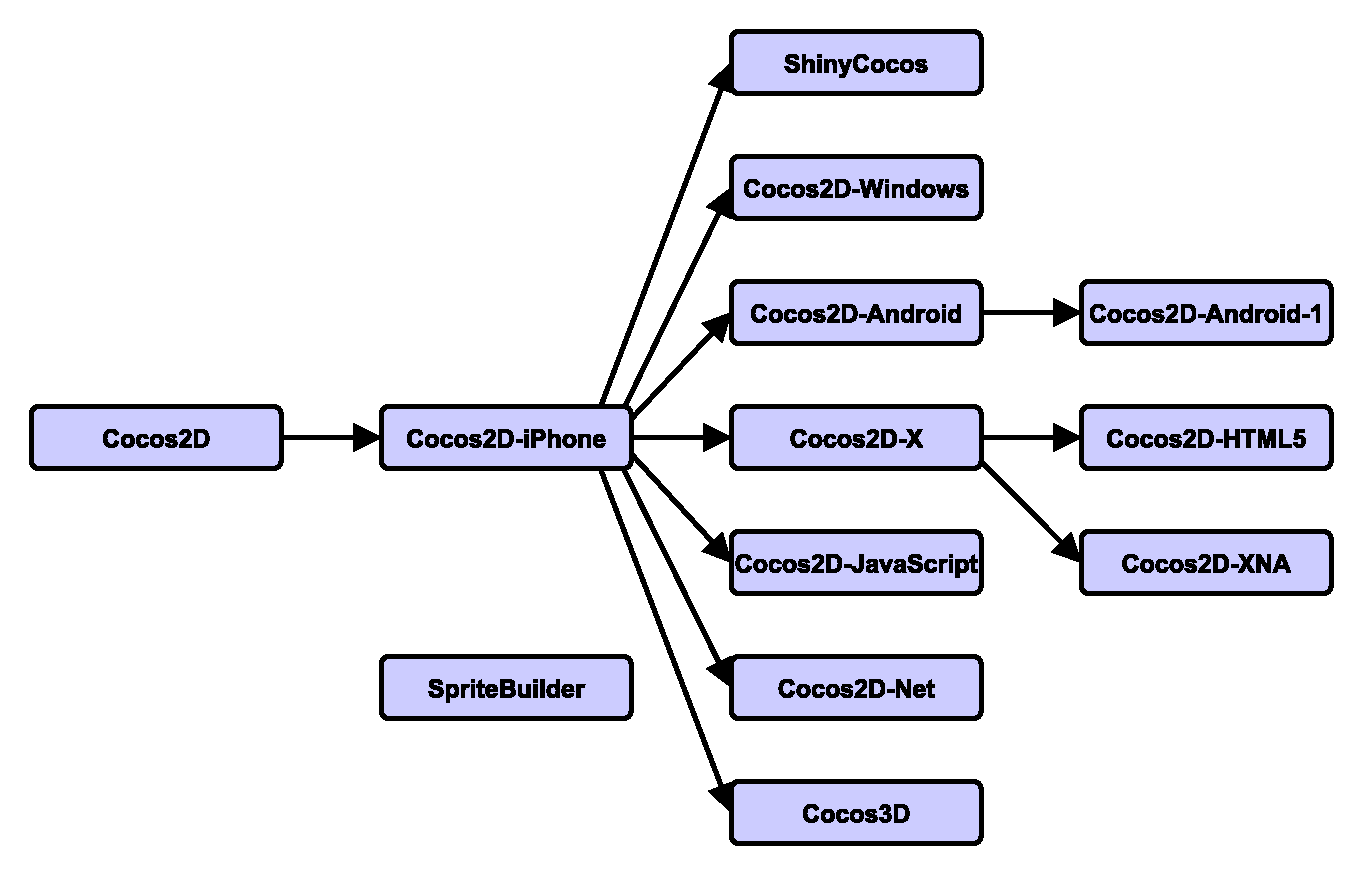
\includegraphics[width=1\textwidth]{Bilder/Cocos2d_Relationships}
	\caption{Ableitungen und Varianten von Cocos2D}\label{graph_Cocos2d_Relationships}\citep{cocos2d_relationships}
\end{figure}

\bigskip
\textbf{Unity3D} bietet zwei verschiedene Hauptprodukte an, die Personal und die Professional Edition. Bei der Personal Edition handelt es sich um eine frei verfügbare Version, die für jeden zugängig ist. Diese kann für Privatanwender, zu Bildungszwecken und sogar für die kommerzielle Entwicklung benutzt werden. Die kostenfreie Version der Engine verfügt auch über alle essentiellen Funktionen. Sobald die allgemeinen Einnahmen einer Person oder eines Unternehmens mehr als 100.000 US-Dollar aus dem Vorjahr betragen, besteht die Verpflichtung auf die Professional Edition zu wechseln. In dieser bekommt man dann auch die Option auf zusätzliche Funktionen, wie Analyse Tools und die Möglichkeit Projekte in einer speziellen Cloud zu veröffentlichen. In Tabelle \ref{Unity_Produkte} werden die Möglichkeiten beider Editionen gegenübergestellt. Das Kostenmodell beginnt derzeit mit einem Abonnement von 75 US-Dollar pro Monat oder einer Einmalzahlung von 1.500 US-Dollar. Die mit der Einmalzahlung erworbene Dauerlizenz gilt allerdings nur für die aktuelle Version und deren Updates. Das bedeutet bei dem Erwerb von Unity Pro 5 hat man nicht automatisch die Nutzungsrechte für die darauf folgende Version 6. Diese müssten dann in Form eines kostenpflichtigen Upgrades erfolgen. Weitere optionale Erweiterungen können mit den iOS Pro und Android Pro Add-Ons erworben werden, die weitere Funktionen zur Personalisierung ermöglichen. Zusätzliche kostenpflichtige Pakete sind die professionelle Unterstützung bei Projekten oder der Zugang zum Quellcode der Engine. \citep{unity_products}

\begin{table}[htbp]
	\centering
	\resizebox{\textwidth}{!}{%
		\begin{tabular}{cc}
			\rowcolor[HTML]{000000} 
			{\color[HTML]{FFFFFF} \textbf{Edition}} & {\color[HTML]{FFFFFF} \textbf{Feature}}                                                                                               \\
			Professional / Personal                 & Game Engine inklusive aller Funktionen                                                                                                \\
			\rowcolor[HTML]{C0C0C0} 
			Professional / Personal                 & \begin{tabular}[c]{@{}c@{}}Unterstützung aller Plattformen\\ (ohne Zusatzlizenz Unity Splash Screen bei iOS und Android)\end{tabular} \\
			Professional / Personal                 & Lizenzfreiheit                                                                                                                        \\
			\rowcolor[HTML]{C0C0C0} 
			Professional                            & Unity Cloud Building                                                                                                                  \\
			Professional                            & Team Lizenz                                                                                                                           \\
			\rowcolor[HTML]{C0C0C0} 
			Professional                            & Game Performance Analyse                                                                                                              \\
			Professional                            & Keine Einkommensbeschränkung                                                                                                          \\
			\rowcolor[HTML]{C0C0C0} 
			Professional                            & Personalisierbarer Splash Screen                                                                                                      \\
			Professional                            & Unity Analytics zur Analyse des Spielerverhaltens                                                                                     \\
			\rowcolor[HTML]{C0C0C0} 
			Professional                            & Priorisierte Behandlung bei eingereichten Bugs                                                                                        \\
			Professional                            & Zugang zu Beta-Versionen                                                                                                              \\
			\rowcolor[HTML]{C0C0C0} 
			Professional                            & Unterstützung für zukunftige Plattformen                                                                                              \\
			Professional                            & Vergünstigungen im Asset Store                                                                                                       
		\end{tabular}
	}
	\caption{Gegenüberstellung von Personal und Professional Edition}
	\label{Unity_Produkte}\citep{unity_products}
\end{table}

%OPTIONAL: Vergleichstabelle
%\section{Kosten-Nutzen Vergleich}
%Vergleichstabelle zu den Variationen der Projektanforderungen im Zusammenhang mit den Möglichkeiten und Kosten der Frameworks

%OPTIONAL!!!
%\chapter{Analyse der Marktanteile}
%\section{Menge an Firmen und Entwicklern}
%\section{Menge an Games}


%OPTIONAL!!!
%\chapter{Grundgerüst und Aufbau eines Cross-Plattform Projekts}
%\section{Geteilter Content}
%\section{Plattformabhängiger Content}
%\section{Grundaufbau bei Engines}
%\section{Grundaufbau bei Frameworks}

%OPTIONAL!!!
%\chapter{Game-typische Design Patterns und Architekturen}
%\section{Architekturen}
%\section{Patterns}
%\section{Verweis auf Bachelorarbeit: „Use of Design Patterns for mobile game Development“}


%TODO: Kapitel 13
\chapter{Konzeption und Implementierung einer Beispiel-Applikation}
Um die Möglichkeiten der gewählten Entwicklungstools tiefgehender analysieren zu können, sollten die theoretischen Informationen um praktische Erkenntnisse ergänzt werden. Demnach wird als Teil dieser Arbeit ein Beispiel-Spiel konzipiert, mit den jeweiligen Tools umgesetzt und daraus Applikationen für verschiedene Plattformen erzeugt. Die Anwendung soll dann Anhand von vereinbarten Metriken bemessen und analysiert werden. Die gewonnenen Resultate werden daraufhin in Zusammenhang mit den theoretischen Informationen komplementiert und die Entwicklungstools als Ganzes verglichen. 

\section{Definition von Anforderungen}
\label{sec:definition_anforderungen}
Applikationen aus den Kategorien Business, Unterhaltung und die meisten weiteren ohne den Fokus auf Spiele, greifen in der Regel auf plattformspezifische Benutzeroberflächen zurück. Native Apps besitzen jeweils technische und optische Konventionen. Cross-Plattform Apps versuchen diese möglichst genau zu generieren und einzuhalten, um dem Benutzer ein natives Look-and-Feel zu bieten. 
Meist folgen Spiele diesen Regeln nicht, da sie in Abhängigkeit des Spielprinzips auf unterschiedliche Eingabeelemente und UIs zurückgreifen. 
Das Spiel als solches ist ein komplexes Phänomen, mit dem sich bereits Philosophen, Psychologen, Philanthropen und Forscher aus anderen Fachgebieten auseinandergesetzt haben. Ein Teilbereich der Spielwissenschaft, genannt Ludologie (Die Lehre über das Spiel), befasst sich unter anderem mit der Erforschung des digitalen Spielens. \citep{ludologie} Die Forschungsinhalte befassen sich unter anderem mit Fragestellungen aus den Bereichen:

\begin{itemize}
	\item Geschichte des digitalen Spielens
	\item Elemente des digitalen Spiels
	\item Begrifflichkeit zur Klassifizierung von Spielen und Genres
	\item Regeln und Spielmechanik
	\item u.v.m.
\end{itemize}


Wie definiert man aber nun den Inhalt und den Umfang eines Computerspiels?
Um sich in den konkurrierenden Theorien zu verlieren, wird hierfür beispielhaft die Gebrauchsdefinitionen von Salen und Zimmerman herangezogen:

\bigskip
\emph{„A game is a system in which players engage in an artificial conflict, defined by rules, that results in a quantifiable outcome.”} \citep[80]{salen_zimmerman}
\bigskip

Aus dieser Definition lassen sich einige wesentliche Konzepte entnehmen.

\bigskip
\textbf{Spieler}\\
Ein Spiel ist etwas, das ein oder mehrere Spieler aktiv spielen. Die Spieler interagieren mit dem System und Methoden des Spiels.

\bigskip
\textbf{Konflikt}\\
Der Konflikt bezeichnet den Wettkampfcharakter jedes Spiels. Dieser kann verschiedene Formen annehmen, wie kompetitive Elemente oder der Konflikt gegen das Spielsystem. 

\bigskip
\textbf{Regeln}\\
Die Regeln liefern die Struktur des Spiels, in dem sie festlegen was der Spieler machen kann und was nicht.

\bigskip
\textbf{Quantifizierbares Ziel}\\
Das Ergebnis eines Spiels ist entweder das der Spieler gewonnen oder verloren hat, oder eine Form eines Erfolgsfaktors erhält. Dieser Erfolgsfaktor kann sich beispielsweise durch ein höheres Level oder eine Art Punktzahl bemerkbar machen. 
\citep[80]{salen_zimmerman}

\bigskip
Anhand dieser Definitionen werden die Anforderungen für die Beispielapplikation konkretisiert:

\begin{itemize}
	\item Es soll eine Spielfigur geben, auf die der Spieler Einfluss nehmen kann.
	\item Die Spielfigur soll auf Hindernisse treffen, welche die Aktionen des Spielers beeinflussen können.
	\item Der Spieler gewinnt, wenn er ein definiertes Ziel erreicht oder das Spiel nicht beendet wird.
	\item Der Spieler verliert, wenn er eine definierte Anzahl an Fehlversuchen erreicht hat, das Spiel abbricht oder andere Aktionen ausführt, die gegensätzlich zum gewinnen des Spiels stehen.
	\item Der Spieler soll einen Erfolgsfaktor erhalten, um seine Spielweise zu messen.
\end{itemize}

Darüber hinaus werden weitere allgemeine Anforderungen gestellt, die häufig in Spielen enthalten sind:

\begin{itemize}
	\item Das Spiel soll einen visuellen Charakter haben und Grafiken verwenden.
	\item In dem Spiel sollen Animationen vorkommen, wie Bewegungen. 
	\item Das Spiel soll über Audioelemente verfügen, wie Musik oder Soundeffekte.
	\item Es sollen mehrere Spielszenen verwendet werden.
	\item Ein Spielobjekt soll in allen Szenen verfügbar sein und seinen Status beibehalten.
\end{itemize}

Die Applikation soll zudem möglichst simpel gehalten werden, um sie Anhand der einfachsten und elementaren Eigenschaften zu bemessen.


\section{Spielidee}
Ein mobiles Spiel das mitunter durch seine Einfachheit, in kürzester Zeit großen Erfolg erlangte, ist das Spiel Flappy Bird. \citep{flappy_bird}
In diesem Spiel steuert der Spieler durch Antippen des Touchscreens die Flughöhe eines Vogels, um ihn vor dem Aufprall auf den Boden zu bewahren und durch entgegenkommende Hindernisse zu manövrieren. Hierbei handelt es sich um eine Art Endlos-Spiel, das sich dadurch auszeichnet, dass der Spieler solange spielt, bis er verliert. Verlieren kann man, indem die Spielfigur mit einem anderen Objekt kollidiert. Es verfügt zudem über eine Punktzahl, die sich erhöht, wenn der Vogel erfolgreich die Hindernisse passiert hat.

\bigskip
In der Anlehnung zu Flappy Bird entstanden zahlreiche Spiele die große Ähnlichkeit aufweisen. Auch wird dieses Spielprinzip häufig als Vorlage verwendet, um beispielhaft den Einstieg in die Spielentwicklung mit einer bestimmten Engine oder einem Framework zu erlernen. Da alle vorher genannten Anforderungen in dieses Spielprinzip hineinpassen, wurde für diese Arbeit ein Spiel konzipiert, das sich an dieser Vorlage orientiert. Das Spiel trägt den Titel: \textbf{Happy Bird}. 

\section{Spielfluss}
Das Spielprinzip und der Spielfluss bei Happy Bird sind denkbar einfach. Das Spiel wurde zudem auf den Portrait-Modus (Hochformat) festgelegt und es wird durchgängig eine Anzeige mit der aktuellen Framerate dargestellt.


\begin{enumerate}
	\item Das Spiel wird über das App Icon gestartet.
	\item Direkt nach dem Start wird ein Logo des jeweiligen Frameworks oder Engine angezeigt.
	\item Daraufhin gelangt man in ein Hauptmenü, das den Titel des Spiels, Hintergrundgrafiken und einen Startbutton anzeigt. Die Hintergrundmusik wird abgespielt.
	\item Bei betätigen des Startbuttons wird in die Spielszene gewechselt.
	\item Die Spielszene beginnt mit den Hintergrundgrafiken und einem Vogel als Spielfigur.
	\item Der Vogel verliert an Höhe, wenn der Spieler nichts tut und steigt bei antippen des Touchscreens an.
	\item In einem festgelegten Intervall kommen der Figur nun Hindernisse in Form von grünen Röhren entgegen. Diese besitzen eine Lücke in der Mitte, durch die der Vogel hindurchmanövriert werden muss. Die Position der Lücke befindet sich in einer zufälligen, vertikalen Stelle innerhalb der Sichtbarkeit.
	\item Wenn der Vogel erfolgreich das Hindernis passiert hat, erhält man einen Punkt, der oben links im Spiel zu der Gesamtpunktzahl hinzugefügt und dargestellt wird.
	\item Das Spiel endet und gilt als verloren, wenn der Vogel mit einem der entgegenkommenden Hindernisse oder dem Boden kollidiert.
	\item Der obere Rand der Spielszene wird durch eine unsichtbare Wand blockiert, die nicht passiert werden kann.
	\item Bei verlorenem Spiel, wird in das Game Over Menü gewechselt, das wie das Hauptmenü aufgebaut ist. Dies zeigt den Game Over Status an und gibt die Möglichkeit, über den Startbutton ein neues Spiel zu starten.
\end{enumerate}

%TODO: Screenshots! Spielszenen / alle Frameworks / verschiedene Geräte


Die in Kapitel \ref{sec:definition_anforderungen} definierten Anforderungen, werden somit alle umgesetzt. Die Spielfigur wird durch einen Spritesheet animiert und ist durch Touchscreen-Input steuerbar. Es werden Hindernisse erzeugt, die bei Kollision das Spielende hervorrufen. Der Spieler hat die Möglichkeit Punkte zu erhalten.
Die Hintergrundmusik wird in allen drei Spielszenen gespielt. Sie startet bei Wechsel der Szene nicht von vorne, behält einen globalen Status bei und wird in einer Endlosschleife gespielt. Das Spiel wird komplett in 2D gehalten. Auf weitere diverse, für eine Testapplikation unnötige Benutzerannehmlichkeiten wurde verzichtet. Für die Versionierung der Projekte wird Git verwendet.


\section{Verwendete Werkzeuge}
In diesem Kapitel werden die genutzten Softwarewerkzeuge in Tabell \ref{genutzte_software} aufgelistet, die bei der Entwicklung der Testapplikation eingesetzt wurden.

\begin{table}[htbp]
	\centering
	\resizebox{0.8\textwidth}{!}{%
		\begin{tabular}{ccc}
			& \cellcolor[HTML]{000000}{\color[HTML]{FFFFFF} \textbf{Betriebssystem}} & \cellcolor[HTML]{000000}{\color[HTML]{FFFFFF} \textbf{Version}}                  \\
			\cellcolor[HTML]{000000}{\color[HTML]{FFFFFF} \textbf{Betriebssysteme}}                                                  &                                                                        &                                                                                  \\
			\textbf{Mac OS X}                                                                                                        & Mac OS X                                                               &                                                                                  \\
			\rowcolor[HTML]{C0C0C0} 
			\textbf{Windows}                                                                                                         & Windows                                                                & \begin{tabular}[c]{@{}c@{}}Windows 8.1\\  Standard Edition\\ 64-Bit\end{tabular} \\
			\cellcolor[HTML]{000000}{\color[HTML]{FFFFFF} \textbf{\begin{tabular}[c]{@{}c@{}}Game-\\ Framework/Engine\end{tabular}}} &                                                                        &                                                                                  \\
			\textbf{libGDX}                                                                                                          & \begin{tabular}[c]{@{}c@{}}Mac OS X,\\ Windows\end{tabular}            &                                                                                  \\
			\rowcolor[HTML]{C0C0C0} 
			\textbf{Cocos2D-X}                                                                                                       & \begin{tabular}[c]{@{}c@{}}Mac OS X,\\ Windows\end{tabular}            &     3.9                                                                             \\
			\textbf{Unity3D}                                                                                                         & \begin{tabular}[c]{@{}c@{}}Mac OS X,\\ Windows\end{tabular}            & 5.3.2f1                                                                          \\
			\cellcolor[HTML]{000000}{\color[HTML]{FFFFFF} \textbf{Programmiersprache}}                                               &                                                                        &                                                                                  \\
			\textbf{Java}                                                                                                            & \begin{tabular}[c]{@{}c@{}}Mac OS X,\\ Windows\end{tabular}            &                                                                                  \\
			\rowcolor[HTML]{C0C0C0} 
			\textbf{C++}                                                                                                             & \begin{tabular}[c]{@{}c@{}}Mac OS X, \\ Windows\end{tabular}           &                                                                                  \\
			\textbf{C\#}                                                                                                             & \begin{tabular}[c]{@{}c@{}}Mac OS X, \\ Windows\end{tabular}           &                                                                                  \\
			\rowcolor[HTML]{C0C0C0} 
			\textbf{Objective-C}                                                                                                     & Mac OS X                                                               &                                                                                  \\
			\textbf{Python}                                                                                                          & \begin{tabular}[c]{@{}c@{}}Mac OS X, \\ Windows\end{tabular}           &                                                                                  \\
			\cellcolor[HTML]{000000}{\color[HTML]{FFFFFF} \textbf{Entwicklungsumgebung}}                                             &                                                                        &                                                                                  \\
			\textbf{Xcode}                                                                                                           & Mac OS X                                                               &                                                                                  \\
			\rowcolor[HTML]{C0C0C0} 
			\textbf{Android Studio}                                                                                                  & \begin{tabular}[c]{@{}c@{}}Mac OS X, \\ Windows\end{tabular}           &                                                                                  \\
			\textbf{Visual Studio}                                                                                                   & Windows                                                                &                                                                                  \\
			\rowcolor[HTML]{C0C0C0} 
			\textbf{Monodevelop}                                                                                                     & \begin{tabular}[c]{@{}c@{}}Windows, \\ Mac OS X\end{tabular}           &                                                                                  \\
			\cellcolor[HTML]{000000}{\color[HTML]{FFFFFF} \textbf{Sonstiges}}                                                        &                                                                        &                                                                                  \\
			\textbf{Android SDK}                                                                                                     & \begin{tabular}[c]{@{}c@{}}Mac OS X,\\ Windows\end{tabular}            &                                                                                  \\
			\rowcolor[HTML]{C0C0C0} 
			\textbf{Android NDK}                                                                                                     & \begin{tabular}[c]{@{}c@{}}Mac OS X,\\ Windows\end{tabular}            &                                                                                  \\
			\textbf{Android ANT}                                                                                                     & \begin{tabular}[c]{@{}c@{}}Mac OS X,\\ Windows\end{tabular}            &                                                                                  \\
			\rowcolor[HTML]{C0C0C0} 
			\textbf{Mono}                                                                                                            & \begin{tabular}[c]{@{}c@{}}Mac OS X, \\ Windows\end{tabular}           &                                                                                  \\
			\textbf{RoboVM}                                                                                                          & \begin{tabular}[c]{@{}c@{}}Mac OS X, \\ Windows\end{tabular}           &                                                                                 
		\end{tabular}
	}
	\caption{Eingesetzte Software auf den jeweiligen Betriebssystemen und Versionen}\label{genutzte_software}
\end{table}

\section{Eingesetzte Komponenten}
\label{sec:eingesetze_komponenten}
Bei den eingesetzten und benötigten Komponenten existieren geringe Unterschiede. Um eine Sprite-Animation in Cocos2D und libGDX zu ermöglichen, empfehlen die Frameworks die Nutzung von Spritesheets in Kombination mit einer Property List-Datei (.plist). Bei einem Spritesheet handelt es sich um eine Sammlung von Grafiken in einer Datei. Diese Grafiken können allein oder in einer zusammenhängenden Abfolge stehen. Diese werden dann der Größe entsprechend ausgeschnitten.

\begin{figure}[htbp]
	\centering
	
\includegraphics[width=1.0\textwidth]{bilder/Red_Bird}
	\caption{Spritesheet für die Animation der Spielfigur in Happy Bird}\label{spritesheet}
\end{figure}

Durch Zuhilfenahme der Property List (Liste von Eigenschaften), die in Zusammenhang mit dem Spritesheet erstellt werden kann, können Informationen über die einzelnen Sprites ausgelesen werden. Diese geben Auskunft über Namen, Größe, Offset, Skalierung und Rotation der einzelnen Grafiken auf dem Spritesheet und sind auf Basis von XML-Dateien gespeichert oder binär kodiert. Innerhalb der Anwendung können die einzelnen Grafiken dann in einer einstellbaren Geschwindigkeit und Dauer nacheinander angezeigt werden. Diese Art von Animation ähnelt einem Daumenkino.
In Unity3D können ebenfalls Spritesheets genutzt werden, jedoch werden die Property Lists für die Teilung und den Informationshintergrund nicht benötigt. Komfortable Möglichkeiten bieten die sogenannten Prefabs. Ein Prefab kann spezifisch definierte Informationen und Eigenschaften über ein oder mehrere Gameobjekte tragen und diese in einem Objekt abrufbereit verfügbar machen. In Happy Bird werden die Pipe-Hindernisse beispielsweise als Prefab definiert, mit dem Inhalt der Grafiken, der Positionen und der Kollisionsboxen.
Für die Erstellung der Grafiken und Animationen wurde der freie Online-Spriteeditor Piskel verwendet. \citep{piskel}
Die genutzte Hintergrundmusik in Happy Bird, stammt von dem amerikanischen Komponisten und Musikproduzenten Kevin MacLeod. Das Musikstück mit dem Titel \emph{"Monkeys Spinning Monkeys"} ist unter der Creative Commons lizensiert und frei verfügbar. \citep{macLeod}
In Tabelle \ref{spiel_komponenten} werden die Hauptkomponenten und ihre Eigenschaften, sowie einige Framework-abhängige Dateien aufgelistet.

\begin{table}[htbp]
	\centering
	\resizebox{\textwidth}{!}{%
		\begin{tabular}{ccccc}
			\rowcolor[HTML]{000000} 
			{\color[HTML]{FFFFFF} Dateiname}   & {\color[HTML]{FFFFFF} Dateityp} & {\color[HTML]{FFFFFF} Objekttyp}     & {\color[HTML]{FFFFFF} Verwendung}       & {\color[HTML]{FFFFFF} Dateigröße (KB)} \\
			{\color[HTML]{000000} Red\_Bird}   & {\color[HTML]{000000} PNG}      & {\color[HTML]{000000} Spritesheet}   & {\color[HTML]{000000} Spielfigur}       & {\color[HTML]{000000}1,54}           \\
			\rowcolor[HTML]{C0C0C0} 
			{\color[HTML]{000000} bird}        & {\color[HTML]{000000} PLIST}    & {\color[HTML]{000000} Property List} & {\color[HTML]{000000} Spielfigur}       & {\color[HTML]{000000}2,94}           \\
			{\color[HTML]{000000} sprite\_1}   & {\color[HTML]{000000} PNG}      & {\color[HTML]{000000} Sprite}        & {\color[HTML]{000000} Spielfigur}       & {\color[HTML]{000000}0,44}           \\
			\rowcolor[HTML]{C0C0C0} 
			{\color[HTML]{000000} sprite\_2}   & {\color[HTML]{000000} PNG}      & {\color[HTML]{000000} Sprite}        & {\color[HTML]{000000} Spielfigur}       & {\color[HTML]{000000}0,4}           \\
			{\color[HTML]{000000} sprite\_3}   & {\color[HTML]{000000} PNG}      & {\color[HTML]{000000} Sprite}        & {\color[HTML]{000000} Spielfigur}       & {\color[HTML]{000000}0,39}           \\
			\rowcolor[HTML]{C0C0C0} 
			{\color[HTML]{000000} sprite\_4}   & {\color[HTML]{000000} PNG}      & {\color[HTML]{000000} Sprite}        & {\color[HTML]{000000} Spielfigur}       & {\color[HTML]{000000}0,4}           \\
			{\color[HTML]{000000} Sky}         & {\color[HTML]{000000} PNG}      & {\color[HTML]{000000} Sprite}        & {\color[HTML]{000000} Hintergrund}      & {\color[HTML]{000000}11,8}           \\
			\rowcolor[HTML]{C0C0C0} 
			{\color[HTML]{000000} Ground}      & {\color[HTML]{000000} PNG}      & {\color[HTML]{000000} Sprite}        & {\color[HTML]{000000} Hindernis}        & {\color[HTML]{000000}3,05}           \\
			{\color[HTML]{000000} Pipe}        & {\color[HTML]{000000} PNG}      & {\color[HTML]{000000} Sprite}        & {\color[HTML]{000000} Hindernis}        & {\color[HTML]{000000}1,99}           \\
			\rowcolor[HTML]{C0C0C0} 
			{\color[HTML]{000000} StartButton} & {\color[HTML]{000000} PNG}      & {\color[HTML]{000000} Sprite}        & {\color[HTML]{000000} Button}           & {\color[HTML]{000000}6,98}           \\
			{\color[HTML]{000000} Marker Felt} & {\color[HTML]{000000} TTF}      & {\color[HTML]{000000} Font}          & {\color[HTML]{000000} Schrift}          & {\color[HTML]{000000}26}           \\
			\rowcolor[HTML]{C0C0C0} 
			{\color[HTML]{000000} Arial}       & {\color[HTML]{000000} TTF}      & {\color[HTML]{000000} Font}          & {\color[HTML]{000000} Schrift}          & {\color[HTML]{000000}761}           \\
			{\color[HTML]{000000} BGMusic}     & {\color[HTML]{000000} MP3}      & {\color[HTML]{000000} Audio}         & {\color[HTML]{000000} Hintergrundmusik} & {\color[HTML]{000000}4770}          
		\end{tabular}
	}
	\caption{Liste von eingesetzten Spielelementen und deren Eigenschaften}
	\label{spiel_komponenten}
\end{table}

\section{Programmierung}
Für die Entwicklung wurde C++ bei Cocos2D-X, C\# bei Unity3D und Java bei libGDX für die Codebasis gewählt. Dies liegt darin begründet, dass diese objektorientierten, statisch typisierten Sprachen im Gegensatz zu den Skriptsprachen eine bessere Performance versprechen. Jedoch mit welcher Programmiersprache man die schnellsten und effizientesten Ergebnisse erzielen kann, steht zusätzlich in Verbindung mit der subjektiven Vorerfahrung.
Während des Entwicklungsprozesses bestätigte sich ein weiterer wichtiger Faktor. Die Qualität der Dokumentation und Codebeispiele der Spieleframeworks. 

\bigskip
Für libGDX finden sich viele Beispiele zu verschiedenen Bereichen innerhalb des offiziellen Wiki, die funktional sind und zudem mit Texten zur Erklärung hinterlegt sind. Auch die Suche nach individuelleren Lösungen wird befriedigend gesättigt. Die Entwicklungsgeschwindigkeit ist für jemanden ohne Vorerfahrung von daher durchaus annehmbar.

\bigskip
In diesem Punkt enttäuschte Cocos2D leider mehr als zuvor angenommen. Die offizielle Dokumentation schwächelt an vielen grundlegenden Stellen bezüglich der Aktualität. Dies muss nicht unbedingt tragisch sein, jedoch sind manche Einträge zu Standardlösungen nicht mehr ganz aktuell und lassen sich nicht mehr wie beschrieben anwenden. Das gleiche gilt für allgemeine Suchanfragen für Lösungen im Internet. Es ist als Anfänger von daher nicht trivial, für manche scheinbar einfache Problemstellungen herauszufinden, was die beste, empfohlene Vorgehensweise sein soll.

\bigskip
Im Gegensatz dazu, macht Unity3D es einem leichter. Einen Neuling mag dieser umfangreiche Editor zunächst mehr fordern, hingegen werden für jede Erfahrungsstufe Hilfestellungen geboten. Die Vielfalt an Unterstützung ist immens, fast immer mit praktischen Beispielen vertieft und gut sortiert. Wenn es passiert, dass überholte Methoden verwendet werden, hilft einem die unterstützte IDE oder die Dokumentation sofort weiter. Ein weiterer Vorteil und Zeitersparnis ist das direkte testen des Spiels innerhalb des Unity Editors. Das Testspiel konnte somit ohne Hindernisse umgesetzt werden.


%TODO
\chapter{Analyse der Test-Applikationen}

%TODO: Auf Analyse der Frameworks eingehen
\section{Definition von Metriken}
Die erstellten Applikationen sollen näher analysiert werden. Um dies möglichst objektiv und repräsentativ durchzuführen, müssen vergleichbare Metriken definiert werden.
Gleichfalls muss für jede Metrik der Ablauf der Messung, sowie der Ausgangszustand der Testgeräte normiert werden.

\bigskip
\textbf{Gesamtgröße einer Basisapplikation} \\
Mit Basisapplikation ist die Anwendung gemeint, die bei Anlegung eines neuen Projekts erzeugt wird. Dies ist in der Regel eine App mit einer Szene / View und wird oft als \emph{Hello World} deklariert. Dies soll eine Vorstellung über die Grundgröße einer minimalen Applikation geben und die Gesamtgröße des Spiels verständlicher darstellen. Für die Messung wird jeweils ein neues Projekt angelegt, daraus Applikationen erzeugt und die Dateigröße auf dem Testgerät dokumentiert. Ein niedriger Wert gilt als positiv, ein hoher als negativ.

\bigskip
\textbf{Gesamtgröße des Spiels} \\
Hiermit ist die Größe der Applikation insgesamt gemeint. Hier werden alle genutzten Ressourcen, Bibliotheken und sonstige Dateien eingerechnet. Für die Messung werden die Dateigrößen der erzeugten Applikationen auf den Testgeräten dokumentiert. Ein niedriger Wert gilt als positiv, ein hoher als negativ.
%TODO: And actually it's pretty easy to see what's taking all the space, rename the .apk to .zip and unzip it!On iOS rename the .ipa to .zip and unzip it. Then do Show Package Contents on the resulting expanded archive file.

%TODO: Verhältnismäßiger Größenunterschied im Vergleich zur Basisapp in Prozent

\bigskip
\textbf{Größe der Ressourcen} \\
Die Ressourcen für das Spiel sind die in Kapitel \ref{sec:eingesetze_komponenten} deklarierten Komponenten. Hierzu zählen einerseits die Komponenten, die als Schnittmenge in allen Projekten vorkommen, sowie diejenigen die für ein jeweiliges Framework und Engine zusätzlich benötigt oder erzeugt wurden. Für die Messung wird die Größe des Ressourcenordners innerhalb des jeweiligen Projekts dokumentiert. Ein niedriger Wert gilt als positiv, ein hoher als negativ.

\bigskip
\textbf{Benötigter Arbeitsspeicher} \\
Der genutzte Arbeitsspeicher, den das Spiel belegt soll ebenfalls dokumentiert werden. Dies kann auf den Testgeräten allerdings nur schwerlich in Echtzeit geschehen, da hierfür die Applikation verlassen werden muss und die Werte aus den Systemeinstellungen abgelesen werden, während die App nur im Hintergrund aktiv ist. Ein niedriger Wert gilt als positiv, ein hoher als negativ.

\bigskip
\textbf{Ladegeschwindigkeit bei Neustart} \\
Die Ladegeschwindigkeit ist die Zeit zwischen der Betätigung des Starticons und der Bereitschaft der Menüszene. Die Dauer der Anzeige des Splashscreens wurde gemäß der Grundeinstellungen der Projekte übernommen und bildet die Zeit ab, in der die benötigten Dateien geladen werden. Hierfür wird vorausgesetzt, dass die Applikation nicht im Hintergrund aktiv ist. Ein niedriger Wert gilt als positiv, ein hoher als negativ.

\bigskip
\textbf{Frames pro Sekunde} \\
Die Framerate wurde in das Spiel sichtbar in allen Szenen implementiert und innerhalb eines Zeitraums von 15 Minuten beobachtet. Hierbei wird der Durchschnittswert angegeben und eventuelle, auffällige Schwankungen zu bestimmten Zeitpunkten dokumentiert. Ein hoher und zugleich stabiler Wert gilt als positiv, ein niedriger oder stark schwankender als negativ.

\bigskip
\textbf{Akkuverbrauch} \\
Der Akkuverbrauch wird über einen Zeitraum von 15 Minuten gemessen. Ausgangswert ist ein frisch geladenes Testgerät mit 100\% Ladezustand. Das Spiel wird über den Messzeitraum durchgehend genutzt. Dokumentiert wird anschließend der prozentuale Akkuverbrauch. Ein niedriger Wert gilt als positiv, ein hoher als negativ.

\bigskip
\textbf{Geschriebene Zeilen Code} \\
Die Menge der Codezeilen ist nur bedingt eine vergleichbare Metrik, da diese in Abhängigkeit des Programmierstils und der Erfahrung des Entwicklers, der Programmiersprache, der Architektur, des Einsatzes von Kommentaren und der Verwendung von leeren Zeilen abhängt stark beeinflusst wird. Jedoch soll hierdurch ein grober Eindruck über den benötigten Code vermittelt und dokumentiert werden. Für die Zählung werden Kommentare und leere Zeilen ignoriert. Ein niedriger Wert gilt als positiv, ein hoher als negativ.


\section{Testgeräte und Voreinstellungen}
Die Applikationen werden auf Smartphones mit Android und iOS System getestet. Auf eine Analyse des Spiels auf einem Windows Phone wird aus mehreren Gründen verzichtet. libGDX unterstützt die mobilen Windows Systeme derzeit nicht, die aktuellen Betriebssysteme sind nicht kompatibel zueinander, Windows Phone 8 wird nach und nach von Windows 10 abgelöst, weiterhin ist der Marktanteil laut der Analyse relativ gering und von daher vernachlässigbar. Die relevanten Daten der genutzten Testgeräte sind in Tabelle \ref{testgeraete} aufgelistet. Um die zu dokumentierenden Messungen möglichst unverfälscht aufnehmen zu können, werden die Geräte vor der Durchführung der Messung einheitlich konfiguriert. Dies ist notwendig, um Daten wie Akkuverbrauch, Arbeitsspeicher oder Framerate möglichst wenig zu beeinflussen und die Ergebnisse reproduzierbarer zu machen.

\begin{itemize}
	\item Alle Verbindungsoptionen (WLAN, mobiler Datenverkehr, Bluetooth, GPS, …etc.) werden deaktiviert.
	\item Die Bildschirmhelligkeit wird auf 50\% gestellt.
	\item Die Lautstärke für Medien und Anwendungen wird auf 50\% gestellt und alle anderen deaktiviert.
	\item Alle weiteren Anwendungen und Prozesse werden weitestgehend beendet.
	\item Das Gerät wird in den Flug-Modus gesetzt, um die Verbindung zu einem Provider zu unterbinden.
	\item Das Spiel wird auf dem internen Speicher installiert.
\end{itemize}

%TODO: Betriebssystem!
\begin{table}[htbp]
	\centering
	\resizebox{\textwidth}{!}{%
		\begin{tabular}{ccc}
			\rowcolor[HTML]{000000} 
			{\color[HTML]{FFFFFF} \textbf{Technische Daten}}       & {\color[HTML]{FFFFFF} \textbf{Android}}                                                          & {\color[HTML]{FFFFFF} \textbf{iOS}}                                                             \\
			{\color[HTML]{000000} \textbf{Hersteller}}             & {\color[HTML]{000000} Samsung}                                                                   & {\color[HTML]{000000} Apple}                                                                    \\
			\rowcolor[HTML]{C0C0C0} 
			{\color[HTML]{000000} \textbf{Modell}}                 & {\color[HTML]{000000} Galaxy S5+}                                                                & {\color[HTML]{000000} iPhone 4}                                                                 \\
			{\color[HTML]{000000} \textbf{Artikelname}}            & {\color[HTML]{000000} G901F}                                                                     & {\color[HTML]{000000} }                                                                         \\
			\rowcolor[HTML]{C0C0C0} 
			{\color[HTML]{000000} \textbf{Betriebssystem}}         & {\color[HTML]{000000} Android 5.0.2 }                                                                          & {\color[HTML]{000000} }                                                                         \\
			{\color[HTML]{000000} \textbf{System-on-a-Chip (SoC)}} & {\color[HTML]{000000} \begin{tabular}[c]{@{}c@{}}Qualcomm Snapdragon 805\\ APQ8084\end{tabular}} & {\color[HTML]{000000} Apple A4}                                                                 \\
			\rowcolor[HTML]{C0C0C0} 
			{\color[HTML]{000000} \textbf{Prozessor}}              & {\color[HTML]{000000} \begin{tabular}[c]{@{}c@{}}Krait 450\\ 2500 MHz\\ 4 Kerne\end{tabular}}    & {\color[HTML]{000000} \begin{tabular}[c]{@{}c@{}}ARM Cortex A8\\ 800 MHz\\ 1 Kern\end{tabular}} \\
			{\color[HTML]{000000} \textbf{Grafikprozessor}}        & {\color[HTML]{000000} \begin{tabular}[c]{@{}c@{}}Qualcomm Adreno 420\\ 600 MHz\end{tabular}}     & {\color[HTML]{000000} \begin{tabular}[c]{@{}c@{}}PowerVR SGX 535\\ 200 MHz\end{tabular}}        \\
			\rowcolor[HTML]{C0C0C0} 
			{\color[HTML]{000000} \textbf{Arbeitsspeicher}}        & {\color[HTML]{000000} 2 GB}                                                                      & {\color[HTML]{000000} 512 MB}                                                                   \\
			{\color[HTML]{000000} \textbf{Displaygröße}}           & {\color[HTML]{000000} 5,1 Zoll}                                                                  & {\color[HTML]{000000} 3,5 Zoll}                                                                 \\
			\rowcolor[HTML]{C0C0C0} 
			{\color[HTML]{000000} \textbf{Auflösung}}              & {\color[HTML]{000000} 1080 x 1920 Pixel}                                                         & {\color[HTML]{000000} 640 x 960 Pixel}                                                          \\
			{\color[HTML]{000000} \textbf{Akku}}                   & {\color[HTML]{000000} \begin{tabular}[c]{@{}c@{}}2800 mAh\\ Li-Ion\end{tabular}}                 & {\color[HTML]{000000} \begin{tabular}[c]{@{}c@{}}1420 mAh \\ Li-Ion\end{tabular}}              
		\end{tabular}
	}
	\caption{Datenblatt der Android und iOS Testgeräte}
	\label{testgeraete}
\end{table}

Bei den eigesetzten Smartphones handelt es sich um gebrauchte Geräte, was bedeutet, dass manche Leistungsmerkmale zu gleichen Modellen abweichen können. Da es bei Smartphones mit Android und iOS eine sehr große Vielfalt an verschiedensten Geräten, Versionen und Ausstattungen gibt, kann die fehlerfreie Funktion des Spiels nur theoretisch garantiert werden. Um die Darstellung in den unterschiedlichen Auflösungen zu testen, wurden zusätzlich die Simulatoren von Xcode und Android Studio zu Hilfe gezogen.

\section{Messprotokoll}
In diesem Teil der Arbeit werden die Messergebnisse zu den zuvor definierten Metriken, an den angegebenen Testgeräten aufgelistet. In Tabelle \ref{protokoll_android} sind die Ergebnisse der Android Version und in \ref{protokoll_ios} die der iOS Version zu sehen.

%TODO: Kleines Nachwort zu den Ergebnissen. 

\begin{table}[htbp]
	\centering
	\resizebox{\textwidth}{!}{%
		\begin{tabular}{ccccc}
			\rowcolor[HTML]{000000} 
			\multicolumn{5}{c}{\cellcolor[HTML]{000000}{\color[HTML]{FFFFFF} \textbf{Happy Bird - Android}}}                                                                                                                                                                                 \\
			\rowcolor[HTML]{000000} 
			\multicolumn{5}{l}{\cellcolor[HTML]{000000}{\color[HTML]{000000} }}                                                                                                                                                                                                              \\
			\rowcolor[HTML]{000000} 
			{\color[HTML]{FFFFFF} \textbf{Metrik}}                                                                      & {\color[HTML]{FFFFFF} \textbf{Wert}}  & {\color[HTML]{FFFFFF} \textbf{libGDX}} & {\color[HTML]{FFFFFF} \textbf{Cocos2D}} & {\color[HTML]{FFFFFF} \textbf{Unity3D}} \\ \hline
			\multicolumn{1}{|c|}{\textbf{\begin{tabular}[c]{@{}c@{}}Gesamtgröße \\ eines leeren Projekts\end{tabular}}} & \multicolumn{1}{c|}{MB}               & \multicolumn{1}{c|}{}                  & \multicolumn{1}{c|}{}                   & \multicolumn{1}{c|}{}                   \\ \hline
			\multicolumn{1}{|c|}{\textbf{\begin{tabular}[c]{@{}c@{}}Gesamtgröße \\ des Spiels\end{tabular}}}            & \multicolumn{1}{c|}{MB}               & \multicolumn{1}{c|}{}                  & \multicolumn{1}{c|}{}                   & \multicolumn{1}{c|}{}                   \\ \hline
			\multicolumn{1}{|c|}{\textbf{Größe der Ressourcen}}                                                         & \multicolumn{1}{c|}{MB}               & \multicolumn{1}{c|}{}                  & \multicolumn{1}{c|}{}                   & \multicolumn{1}{c|}{}                   \\ \hline
			\multicolumn{1}{|c|}{\textbf{Benötigter Arbeitsspeicher}}                                                   & \multicolumn{1}{c|}{MB}               & \multicolumn{1}{c|}{}                  & \multicolumn{1}{c|}{}                   & \multicolumn{1}{c|}{}                   \\ \hline
			\multicolumn{1}{|c|}{\textbf{\begin{tabular}[c]{@{}c@{}}Ladegeschwindigkeit \\ bei Neustart\end{tabular}}}  & \multicolumn{1}{c|}{Sekunden}         & \multicolumn{1}{c|}{}                  & \multicolumn{1}{c|}{}                   & \multicolumn{1}{c|}{}                   \\ \hline
			\multicolumn{1}{|c|}{\textbf{Frames pro Sekunde}}                                                           & \multicolumn{1}{c|}{Frames / Sekunde} & \multicolumn{1}{c|}{}                  & \multicolumn{1}{c|}{}                   & \multicolumn{1}{c|}{}                   \\ \hline
			\multicolumn{1}{|c|}{\textbf{Akkuverbrauch}}                                                                & \multicolumn{1}{c|}{Prozent / Minute} & \multicolumn{1}{c|}{}                  & \multicolumn{1}{c|}{}                   & \multicolumn{1}{c|}{}                   \\ \hline
			\multicolumn{1}{|c|}{\textbf{}}                                                                             & \multicolumn{1}{c|}{}                 & \multicolumn{1}{c|}{}                  & \multicolumn{1}{c|}{}                   & \multicolumn{1}{c|}{}                   \\ \hline
			\multicolumn{1}{|c|}{\textbf{}}                                                                             & \multicolumn{1}{c|}{}                 & \multicolumn{1}{c|}{}                  & \multicolumn{1}{c|}{}                   & \multicolumn{1}{c|}{}                   \\ \hline
			\multicolumn{1}{|c|}{\textbf{}}                                                                             & \multicolumn{1}{c|}{}                 & \multicolumn{1}{c|}{}                  & \multicolumn{1}{c|}{}                   & \multicolumn{1}{c|}{}                   \\ \hline
			\multicolumn{1}{|c|}{\textbf{}}                                                                             & \multicolumn{1}{c|}{}                 & \multicolumn{1}{c|}{}                  & \multicolumn{1}{c|}{}                   & \multicolumn{1}{c|}{}                   \\ \hline
		\end{tabular}
	}
	\caption{Messprotokoll des Spiels auf Android}\label{protokoll_android}
\end{table}

\begin{table}[htbp]
	\centering
	\resizebox{\textwidth}{!}{%
		\begin{tabular}{ccccc}
			\rowcolor[HTML]{000000} 
			\multicolumn{5}{c}{\cellcolor[HTML]{000000}{\color[HTML]{FFFFFF} \textbf{Happy Bird - iOS}}}                                                                                                                                                                                 \\
			\rowcolor[HTML]{000000} 
			\multicolumn{5}{l}{\cellcolor[HTML]{000000}{\color[HTML]{000000} }}                                                                                                                                                                                                              \\
			\rowcolor[HTML]{000000} 
			{\color[HTML]{FFFFFF} \textbf{Metrik}}                                                                      & {\color[HTML]{FFFFFF} \textbf{Wert}}  & {\color[HTML]{FFFFFF} \textbf{libGDX}} & {\color[HTML]{FFFFFF} \textbf{Cocos2D}} & {\color[HTML]{FFFFFF} \textbf{Unity3D}} \\ \hline
			\multicolumn{1}{|c|}{\textbf{\begin{tabular}[c]{@{}c@{}}Gesamtgröße \\ eines leeren Projekts\end{tabular}}} & \multicolumn{1}{c|}{MB}               & \multicolumn{1}{c|}{}                  & \multicolumn{1}{c|}{}                   & \multicolumn{1}{c|}{}                   \\ \hline
			\multicolumn{1}{|c|}{\textbf{\begin{tabular}[c]{@{}c@{}}Gesamtgröße \\ des Spiels\end{tabular}}}            & \multicolumn{1}{c|}{MB}               & \multicolumn{1}{c|}{}                  & \multicolumn{1}{c|}{}                   & \multicolumn{1}{c|}{}                   \\ \hline
			\multicolumn{1}{|c|}{\textbf{Größe der Ressourcen}}                                                         & \multicolumn{1}{c|}{MB}               & \multicolumn{1}{c|}{}                  & \multicolumn{1}{c|}{}                   & \multicolumn{1}{c|}{}                   \\ \hline
			\multicolumn{1}{|c|}{\textbf{Benötigter Arbeitsspeicher}}                                                   & \multicolumn{1}{c|}{MB}               & \multicolumn{1}{c|}{}                  & \multicolumn{1}{c|}{}                   & \multicolumn{1}{c|}{}                   \\ \hline
			\multicolumn{1}{|c|}{\textbf{\begin{tabular}[c]{@{}c@{}}Ladegeschwindigkeit \\ bei Neustart\end{tabular}}}  & \multicolumn{1}{c|}{Sekunden}         & \multicolumn{1}{c|}{}                  & \multicolumn{1}{c|}{}                   & \multicolumn{1}{c|}{}                   \\ \hline
			\multicolumn{1}{|c|}{\textbf{Frames pro Sekunde}}                                                           & \multicolumn{1}{c|}{Frames / Sekunde} & \multicolumn{1}{c|}{}                  & \multicolumn{1}{c|}{}                   & \multicolumn{1}{c|}{}                   \\ \hline
			\multicolumn{1}{|c|}{\textbf{Akkuverbrauch}}                                                                & \multicolumn{1}{c|}{Prozent / Minute} & \multicolumn{1}{c|}{}                  & \multicolumn{1}{c|}{}                   & \multicolumn{1}{c|}{}                   \\ \hline
			\multicolumn{1}{|c|}{\textbf{Geschriebene Zeilen Code}}                                                                             & \multicolumn{1}{c|}{}                 & \multicolumn{1}{c|}{}                  & \multicolumn{1}{c|}{}                   & \multicolumn{1}{c|}{}                   \\ \hline
			\multicolumn{1}{|c|}{\textbf{}}                                                                             & \multicolumn{1}{c|}{}                 & \multicolumn{1}{c|}{}                  & \multicolumn{1}{c|}{}                   & \multicolumn{1}{c|}{}                   \\ \hline
			\multicolumn{1}{|c|}{\textbf{}}                                                                             & \multicolumn{1}{c|}{}                 & \multicolumn{1}{c|}{}                  & \multicolumn{1}{c|}{}                   & \multicolumn{1}{c|}{}                   \\ \hline
			\multicolumn{1}{|c|}{\textbf{}}                                                                             & \multicolumn{1}{c|}{}                 & \multicolumn{1}{c|}{}                  & \multicolumn{1}{c|}{}                   & \multicolumn{1}{c|}{}                   \\ \hline
		\end{tabular}
	}
	\caption{Messprotokoll des Spiels auf iOS}\label{protokoll_ios}
\end{table}


%\caption{Messprotokoll des Spiels auf Android}\label{protokoll_android}
%Kosten, Performance, Akkuverbrauch, App-Daten-Aufteilung, Größe des benötigten Speichers, Größe des geteilten Contents, Stabilität, RAM, Code-Zeilen/-Größe, Entwicklungszeit(bedingt zu berücksichtigen), FPS

%TODO
\chapter{Vergleich zur Benutzbarkeit}

%TODO
\chapter{Fazit}



%--------------------- VERZEICHNISSE -------------------------------------

\listoffigures % Abbildungsverzeichnis erzeugen
\listoftables % Tabellenverzeichnis erzeugen

%------------------------------ LITERATURVERZEICHNIS----------------------
%TODO:Alphabetisch sortieren!
\begin{thebibliography}{}

\bibitem[Android Develop Tools(2015)]{android_studio}
\emph{Android Studio Overview},
\url{http://developer.android.com/tools/studio/index.html}, letzter Zugriff: 24.11.2015

\bibitem[Android Source - Codenames, Tags, and Build Numbers(2015)]{android_codenames}
\emph{Codenames, Tags, and Build Numbers in the history of Android},
\url{https://source.android.com/source/build-numbers.html}, etzter Zugriff: 24.11.2015

\bibitem[App42(2016)]{app42}
\emph{App42 Cloud API},
\url{http://api.shephertz.com/}, letzter Zugriff: 01.02.2016

\bibitem[Apple Developer(2015)a]{swift_about}
\emph{Swift - Overview},
\url{https://developer.apple.com/swift/}, letzter Zugriff: 28.12.2015

\bibitem[Apple Developer(2016)b]{apple_developer_program}
\emph{How the Program Works},
\url{https://developer.apple.com/programs/how-it-works/}, letzter Zugriff: 15.02.2016

\bibitem[Bernardo Zamora(2015)]{windows_store_trends_2015}
\emph{Blogs.Windows - Windows Store Trends - September 2015},
\url{https://blogs.windows.com/buildingapps/2015/10/12/windows-store-trends-september-2015/}, letzter Zugriff: 15.12.2015

\bibitem[Boo(2015)]{boo_about}
\emph{Boo - A scarily powerful language for .NET},
\url{http://boo-language.github.io/}, letzter Zugriff: 05.01.2016

\bibitem[Brown(2015)]{learning_javascript}
Brown, Ethan (Hrsg.): 
\emph{Learning Javascript}, O'Reilly 2015

\bibitem[Cocos2D-X(2015)a]{cocos2d_main_features}
\emph{Cocos2D-X - Developers Manual},
\url{http://www.cocos2d-x.org/wiki/Cocos2d-x}, letzter Zugriff: 29.12.2015

\bibitem[Cocos2D-X(2015)b]{cocos2d_relationships}
\emph{Cocos2D-X - Relationships in Cocos2D Family},
\url{http://www.cocos2d-x.org/wiki/Relationships_in_Cocos2d_Family}, letzter Zugriff: 05.01.2016

\bibitem[Cocos2D-X(2015)c]{cocos2d_docs}
\emph{Cocos2D-X - Dokumentation},
\url{http://www.cocos2d-x.org/reference/native-cpp/V3.9/index.html}, letzter Zugriff: 10.01.2016

\bibitem[Distimo(2014)]{play_store_categories}
\emph{Anteil der im Google Play Store weltweit am häufigsten heruntergeladenen Apps nach Kategorien im Februar 2014. In Statista - Das Statistik-Portal.},
\url{http://de.statista.com/statistik/daten/studie/321703/umfrage/beliebteste-app-kategorien-im-google-play-store-weltweit/}, letzter Zugriff: 14.12.2015

\bibitem[El-Kassas, Wafaa S. \& Abdullah, Bassem A. \&  Yousef, Ahmed H. \&  Wahba, Ayman M.(2015)]{cross_plattform_approaches} 
El-Kassas, Wafaa S. \& Abdullah, Bassem A. \&  Yousef, Ahmed H. \&  Wahba, Ayman M. :
\glqq Taxonomy of Cross-Platform Mobile Applications Development Approaches\grqq, 
\emph{Ain Shams Engineering Journal}, 2015

\bibitem[Fran Berkman(2012)]{microsoft_mobile}
\emph{Microsoft Mobile: From Pocket PC to Windows Phone 8},
\url{http://mashable.com/2012/10/29/microsoft-mobile-history/#DYxZxZ7wTuqD}, letzter Zugriff: 25.11.2015

\bibitem[Golem(2015)]{wp_with_android_ios}
\emph{Microsoft demonstriert Android- und iOS-Apps unter Windows},
\url{http://www.golem.de/news/windows-10-microsoft-demonstriert-android-und-ios-apps-unter-windows-1504-113812.html}, letzter Zugriff: 25.11.2015

\bibitem[Hölzl \& Raed \& Wirsing(2013)]{java_kompakt}
Hözlz, Matthias \& Raed, Allaithy \& Wirsing, Martin (Hrsg.): 
\emph{Java kompakt Eine Einführung in die Software-Entwicklung
	mit Java}, Springer 2013

\bibitem[IDC(2015)]{marktanteile_betriebssysteme}
\emph{Prognose zu den Marktanteilen der Betriebssysteme am Absatz vom Smartphones weltweit in den Jahren 2015 und 2019. In Statista - Das Statistik-Portal.},
\url{http://de.statista.com/statistik/daten/studie/182363/umfrage/prognostizierte-marktanteile-bei-smartphone-betriebssystemen/}, letzter Zugriff: 14.12.2015

\bibitem[James Whitcomb Riley(1849–1916)]{ducktest}
\emph{Ententest - Begriffsentstehung},
\url{https://de.wikipedia.org/wiki/Ententest}, letzter Zugriff: 05.01.2016

\bibitem[JetBrains(2015)]{appcode}
\emph{AppCode},
\url{https://www.jetbrains.com/objc/}, letzter Zugriff: 28.12.2015

\bibitem[John Daintith(2004)]{native_software}
\emph{A Dictionary of Computing - native software},
\url{http://www.encyclopedia.com/doc/1O11-nativesoftware.html}, letzter Zugriff: 24.11.2015

\bibitem[Junge(2015)]{ludologie}
Junge, Prof. Dr. Jens:
\emph{Zur Begriffsklärung von Ludologie und Spielwissenschaft},
\url{http://www.ludologie.de/neues-spiel/detailansicht/news/detail/News/zur-begriffsklaerung-von-ludologie-und-spielwissenschaft/}, letzter Zugriff: 28.01.2016

\bibitem[Kantar(2015)]{marktanteile_betriebssysteme_laender}
\emph{Marktanteile der mobilen Betriebssysteme am Absatz von Smartphones in ausgewählten Ländern von August bis Oktober 2015. In Statista - Das Statistik-Portal.},
\url{http://de.statista.com/statistik/daten/studie/198453/umfrage/marktanteile-der-smartphone-betriebssysteme-am-absatz-in-ausgewaehlten-laendern/}, letzter Zugriff: 14.12.2015

\bibitem[libGDX(2013)a]{libGDX_main_features}
\emph{libGDX - Goals and Features},
\url{https://libgdx.badlogicgames.com/features.html}, letzter Zugriff: 29.12.2015

\bibitem[libGDX(2013)b]{libGDX_docs}
\emph{libGDX API},
\url{https://libgdx.badlogicgames.com/nightlies/docs/api/}, letzter Zugriff: 10.01.2016

\bibitem[libGDX(2015)c]{libGDX_wiki}
\emph{libGDX - Setting up your Development Environment (Eclipse, Intellij IDEA, NetBeans)},
\url{https://github.com/libgdx/libgdx/wiki/Setting-up-your-Development-Environment-(Eclipse,-Intellij-IDEA,-NetBeans)}, letzter Zugriff: 18.02.2016

\bibitem[Lua(2015)]{lua_about}
\emph{Lua - About},
\url{http://www.lua.org/about.html}, letzter Zugriff: 05.01.2016

\bibitem[Mac Developer Library(2014)]{objectiveC_about}
\emph{About Objective-C},
\url{https://developer.apple.com/library/mac/documentation/Cocoa/Conceptual/ProgrammingWithObjectiveC/Introduction/Introduction.html/}, letzter Zugriff: 28.12.2015

\bibitem[MacinCloud(2015)]{macincloud}
\emph{MacinCloud},
\url{http://www.macincloud.com/}, letzter Zugriff: 28.12.2015

\bibitem[MacLeod(2014)]{macLeod}
MacLeod, Kevin:
\emph{Monkeys Spinning Monkeys},
Licensed under Creative Commons: By Attribution 3.0
http://creativecommons.org/licenses/by/3.0/
\url{http://incompetech.com/music/royalty-free}, letzter Zugriff: 28.01.2016

\bibitem[Microsoft Developer(2015)]{WP10_SDK}
\emph{Windows Software Development Kit (SDK) for Windows 10},
\url{https://dev.windows.com/en-us/downloads/windows-10-sdk}, letzter Zugriff: 28.12.2015

\bibitem[Microsoft(2014)]{microsoft_nokia}
\emph{Microsoft - Microsoft und Nokia Geräte},
\url{https://www.microsoft.com/de-de/nokia.aspx}, letzter Zugriff: 25.11.2015

\bibitem[Microsoft(2015)]{windows10_features}
\emph{Microsoft - Windows 10 Features},
\url{https://www.microsoft.com/de-de/windows/features}, letzter Zugriff: 25.11.2015

\bibitem[MSDN(2015)]{WP10_Emulator}
\emph{Microsoft-Emulator für Windows 10 Mobile},
\url{https://msdn.microsoft.com/library/windows/apps/mt162269.aspx}, letzter Zugriff: 28.12.2015

\bibitem[Nextpeer(2016)]{nextpeer}
\emph{Nextpeer},
\url{https://www.nextpeer.com/}, letzter Zugriff: 01.02.2016

\bibitem[Open Handset Alliance - Alliance Members(2015)]{alliance_members}
\emph{Members of the Open Handset Alliance},
\url{http://www.openhandsetalliance.com/oha_members.html}, letzter Zugriff: 24.11.2015

\bibitem[Open Handset Alliance - Alliance Overview(2015)]{alliance_overview}
\emph{Overview of the Open Handset Alliance},
\url{http://www.openhandsetalliance.com/oha_overview.html}, letzter Zugriff: 24.11.2015

\bibitem[Open Handset Alliance - Android Overview(2015)]{android_overview}
\emph{Overview of Android by the Open Handset Alliance},
\url{http://www.openhandsetalliance.com/android_overview.html}, letzter Zugriff: 24.11.2015

\bibitem[Oracle - Java SE(2015)]{java_jdk}
\emph{Java SE Development Kit 8 Downloads},
\url{http://www.oracle.com/technetwork/java/javase/downloads/jdk8-downloads-2133151.html}, letzter Zugriff: 24.11.2015

\bibitem[Piskel(2015)]{piskel}
\emph{Piskel - Pixel Art and Animated Sprites},
\url{http://www.piskelapp.com/}, letzter Zugriff: 28.01.2016

\bibitem[Play Game Services(2015)]{play_game_services}
\emph{Play Games Services},
\url{https://developers.google.com/games/services/}, letzter Zugriff: 01.02.2016

\bibitem[PocketGamer.biz(2015)]{app_store_categories}
\emph{Ranking der Top-20-Kategorien im App Store im Dezember 2015. In Statista - Das Statistik-Portal.},
\url{http://de.statista.com/statistik/daten/studie/166976/umfrage/beliebteste-kategorien-im-app-store/}, letzter Zugriff: 15.12.2015

\bibitem[Reddit(2015)]{wp_pros_cons}
\emph{Reddit - Pros and cons of Windows phone, and why should I buy one instead of an android or a iPhone?},
\url{https://www.reddit.com/r/windowsphone/comments/3h21lf/pros_and_cons_of_windows_phone_and_why_should_i/}, letzter Zugriff: 25.11.2015

\bibitem[RoboVM(2016)]{roboVM}
\emph{RoboVM - Create truly native iOS apps in Java},
\url{https://robovm.com/}, letzter Zugriff: 15.02.2016

\bibitem[Salen \& Zimmerman(2004)]{salen_zimmerman}
Salen, Katie \& Zimmerman, Eric: 
\glqq Unit 1: Core Concepts: Defining Games\grqq, 
(Hrsg.): \emph{Rules of Play: Game Design Fundamentals}, The MIT Press 2004

\bibitem[Schmidt(2015)]{java_9}
\emph{heise Developer - Java 9: Pläne für Release im Herbst 2016},
\url{http://www.heise.de/developer/meldung/Java-9-Plaene-fuer-Release-im-Herbst-2016-2635526.html}, letzter Zugriff: 06.01.2016

\bibitem[Skeet(2014)]{csharp_in_depth}
Skeet, Jon (Hrsg.): 
\emph{C\# in Depth}, Manning 2014

\bibitem[Statista(2015)]{apps_in_stores}
\emph{Anzahl der angebotenen Apps in den Top App-Stores im Mai 2015. In Statista - Das Statistik-Portal.},
\url{http://de.statista.com/statistik/daten/studie/208599/umfrage/anzahl-der-apps-in-den-top-app-stores/}, letzter Zugriff: 14.12.2015

\bibitem[Sue Smith(2013)]{android_sdk_requirements}
\emph{Android SDK Requirements},
\url{http://code.tutsplus.com/tutorials/android-sdk-requirements--mobile-20086}, letzter Zugriff: 24.11.2015

\bibitem[t3n(2015)]{t3n_xcode7}
\emph{Xcode 7: Apps auch ohne Entwickler-Account auf dem iPhone testen},
\url{http://t3n.de/news/xcode-7-apps-ohne-615214/}, letzter Zugriff: 28.12.2015

\bibitem[techopedia(2015)]{cross_plattform_explanation}
\emph{Cross-Platform Development},
\url{https://www.techopedia.com/definition/30026/cross-platform-development}, letzter Zugriff: 21.12.2015

\bibitem[the iphone wiki(2015)]{ios_codenames}
\emph{iOS Firmwares},
\url{https://www.theiphonewiki.com/wiki/Firmware}, letzter Zugriff: 24.11.2015

\bibitem[Unify Community Wiki(2014)]{unity_unityscript_vs_javascript}
\emph{Unify Community Wiki - UnityScript versus JavaScript},
\url{http://wiki.unity3d.com/index.php/UnityScript_versus_JavaScript}, letzter Zugriff: 05.01.2016

\bibitem[Unity3D(2014)d]{unity_languages}
\emph{Unity3D - Documentation, Unity scripting languages and you},
\url{http://blogs.unity3d.com/2014/09/03/documentation-unity-scripting-languages-and-you/}, letzter Zugriff: 05.01.2016

\bibitem[Unity3D(2015)a]{unity_public_relations}
\emph{Unity3D - Public Relations},
\url{https://unity3d.com/public-relations}, letzter Zugriff: 29.12.2015

\bibitem[Unity3D(2015)b]{unity_managed_plugins}
\emph{Unity3D Documentation - Managed Plugins},
\url{http://docs.unity3d.com/Manual/UsingDLL.html}, letzter Zugriff: 05.01.2016

\bibitem[Unity3D(2015)c]{unity_products}
\emph{Unity3D - Get Unity},
\url{http://unity3d.com/get-unity}, letzter Zugriff: 05.01.2016

\bibitem[Unity3D(2015)d]{unity_docs}
\emph{Unity3D - Scripting API},
\url{http://docs.unity3d.com/ScriptReference/index.html}, letzter Zugriff: 10.01.2016

\bibitem[Unity3D(2016)e]{unity_code_editor}
\emph{Unity3D - Tutorials: Scripting},
\url{https://unity3d.com/learn/tutorials/topics/scripting}, letzter Zugriff: 10.02.2016

\bibitem[Vehse(2014)]{cross_plattform_development_vehse} 
Vehse, Benjamin:
\glqq Plattformabhängige und –unabhängige
Entwicklung mobiler Anwendungen am
Beispiel von Geo-Wikipedia-App\grqq, 
\emph{Bachelor-Thesis}, 2014

\bibitem[Visual Studio(2016)]{visual_studio}
\emph{Visual Studio - Tools für alle Entwickler und alle Apps},
\url{https://www.visualstudio.com/de-de/dn469161}, letzter Zugriff: 15.02.2016

\bibitem[Wikipedia - Flappy Bird(2015)]{flappy_bird}
\emph{Flappy Bird},
\url{https://de.wikipedia.org/wiki/Flappy_Bird}, letzter Zugriff: 28.01.2016

\bibitem[Wikipedia - Liste von Android-Versionen(2015)]{android_version_releases}
\emph{Übersicht von allen Android Versionen mit Veröffentlichungsdatum},
\url{https://de.wikipedia.org/wiki/Liste_von_Android-Versionen}, letzter Zugriff: 24.11.2015

\bibitem[Wikipedia - Windows 10(2015)]{WP10_version_releases}
\emph{Microsoft Windows 10 Mobile},
\url{https://de.wikipedia.org/wiki/Microsoft_Windows_10_Mobile}, letzter Zugriff: 28.12.2015

\bibitem[Wikipedia - Windows Phone 7(2015)]{WP7_version_releases}
\emph{Microsoft Windows Phone 7},
\url{https://de.wikipedia.org/wiki/Microsoft_Windows_Phone_7}, letzter Zugriff: 28.12.2015

\bibitem[Wikipedia - Windows Phone 8(2015)]{WP8_version_releases}
\emph{Microsoft Windows Phone 8},
\url{https://de.wikipedia.org/wiki/Microsoft_Windows_Phone_8}, letzter Zugriff: 28.12.2015

\bibitem[XMLVM(2011)]{XMLVM_Toolchain}
\emph{XMLVM - Overview: Toolchain},
\url{http://xmlvm.org/toolchain/}, letzter Zugriff: 25.12.2015

\bibitem[YoYo Games(2013)]{WP8_requirements}
\emph{Requirements for Windows Phone development},
\url{http://help.yoyogames.com/entries/23355146-Requirements-for-Windows-Phone-development}, letzter Zugriff: 28.12.2015

\end{thebibliography}
%----------------------------- EIGENSTÄNDIGKEITSERKLÄRUNG-----------------
\clearpage\thispagestyle{empty}
\eigen  % im header definiert
%----------------------------- ENDE --------------------------------------
\end{document}